\documentclass{beamer}

\usetheme{CambridgeUS}

\usepackage[utf8x]{inputenc}
\usepackage{tabularx}
\usepackage[romanian]{babel}
\usepackage{natbib}
\usepackage{bibentry}
\usepackage{amsmath}
\usepackage{mathtools}
\usepackage{algorithm}
\usepackage{algorithmic}
\usepackage{graphicx}
\usepackage{caption}
\usepackage{subcaption}

%\usepackage[framed,numbered,autolinebreaks,useliterate]{mcode}



\title[ARIA]{Modele Markov Ascunse}

\subtitle{De la Teorie la Aplicații}

\author[A. Sorici, T. Berariu]{Alexandru Sorici, Tudor Berariu}

\institute[AI-MAS]{Asociația Română pentru Inteligență Artificială}

%% TODO de pus frumos titlurile secțiunilor

%% Autori: Alexandru Sorici, Tudor Berariu
%% Data: Noiembrie 2012

\titlegraphic{
  
\includegraphics[height=.25\textheight]{graphics/branding/aria-logo-small-white.png}
}

%% Numele algoritmului
\floatname{algorithm}{Algoritmul}

%% comandă care trage o linie orizontală (80% din spațiu)
\newcommand{\horiline}{
  \vspace*{-.75em} \begin{center} \begin{tabularx}{.8\linewidth}{
        l } \hline
    \end{tabularx}
  \end{center}
  \vspace*{-.75em}
}

%% comandă pentru frame-uri goale
\newcommand{\dummyframe}{
  \begin{frame}
    \frametitle{De înlocuit} 
    :) 
  \end{frame}
}


%% afișează cuprinsul înainte de fiecare subsecțiune
\AtBeginSubsection[] {
  %\renewcommand\Switch{0}
  \begin{frame}{Outline}
    \tableofcontents[currentsection,currentsubsection,hideallsections]
  \end{frame}
  %\renewcommand\Switch{1}
}



\begin{document}
\maketitle

\begin{frame}
  \tableofcontents[onlyparts]
\end{frame}

\begin{frame}
  \frametitle{Outline}
  \tableofcontents[pausesections]
\end{frame}

\section{Aplicații în Învățarea Automată pentru MMA}
\label{sec:intro-to-hmm}

\subsection{Învățarea Automată}
\label{sec:machine-learning}

%% tudorel
%% Tudor
\begin{frame}
  \frametitle{What is Machine Learning?}
  \begin{block}{Machine Learning}
    A computer program is said to learn from experience $E$ with
    respect to some class of tasks $T$ and performance measure $P$, if
    its performance at tasks in $T$, as measured by $P$, improves with
    experience $E$.
  \end{block}
\end{frame}

\begin{frame}
  \frametitle{Machine Learning Applications}
  \begin{itemize}
  \item Computer Vision: Google Car
  \item Machine Translation
  \item Speech Recognition
  \item Recommender Systems
  \item Intelligent Advertising
  \end{itemize}
\end{frame}

\begin{frame}
  \frametitle{Machine Learning Classification}
  Types of Machine Learning Problems
  \begin{columns}
    \column{0.7\textwidth}
    \begin{itemize}
    \item Regression
    \item Classification
    \item Reinforcement Learning
    \end{itemize}
    \begin{itemize}
    \item supervised learning (eg. ..)
    \item unsupervised
    \end{itemize}
    \column{0.3\textwidth}
    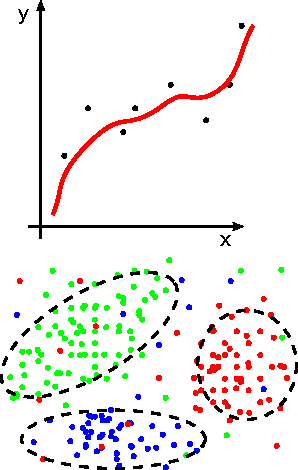
\includegraphics[width=\textwidth]{graphics/ml-intro/ml.pdf}
  \end{columns}
\end{frame}


\subsection{MMA în Învățarea Automată}
\label{sec:hmm-in-ml}

%% alejandro

%% aici facem tranzitie de la problema generala de ML
%% la probleme cu secvente temporale, markov stuff, dbn shit
%% adica HMM-uri :))

%% Markov models, Dynamic Bayesian Networks
\begin{frame}
  \frametitle{Probleme cu Secvențe Temporale (I)}
  \only<1>{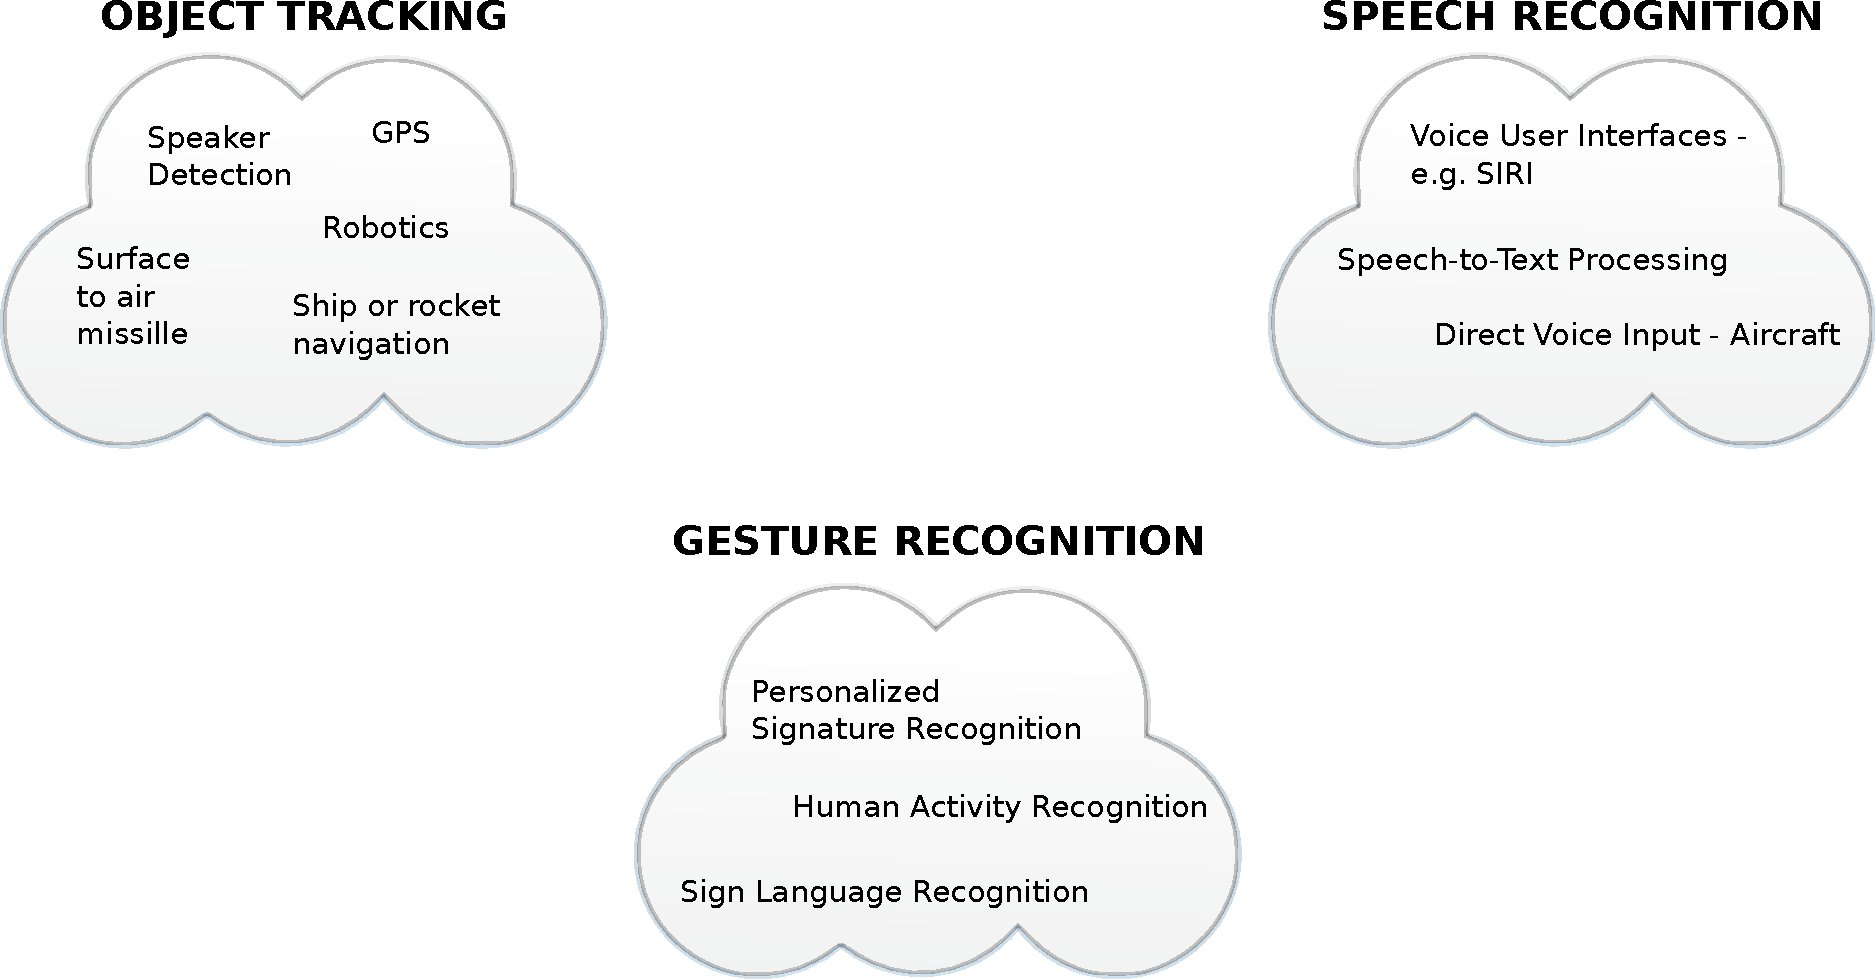
\includegraphics[width=\textwidth]{graphics/hmm-intro/time_series_problems_1.pdf}}
  \only<2>{
  	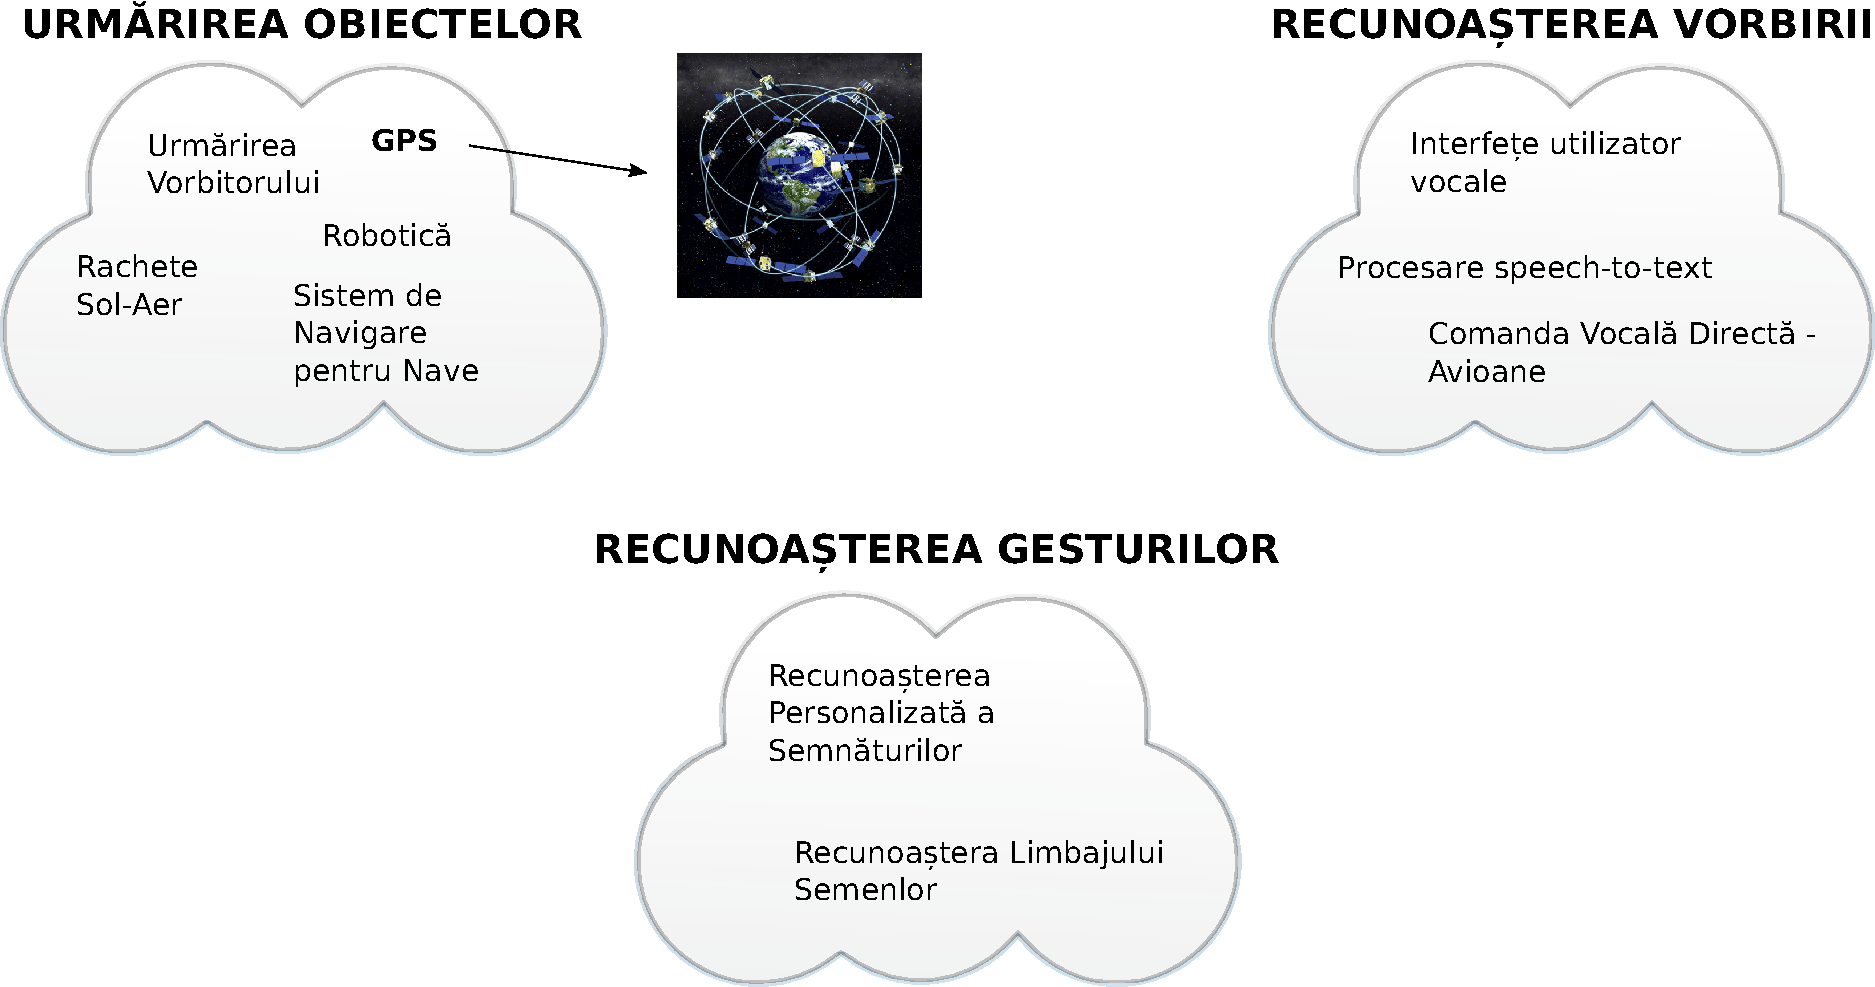
\includegraphics[width=\textwidth]{graphics/hmm-intro/time_series_problems_1_2.pdf}
  	\footnote{Sursa imaginii: Navstar}
  }
  \only<3>{
  	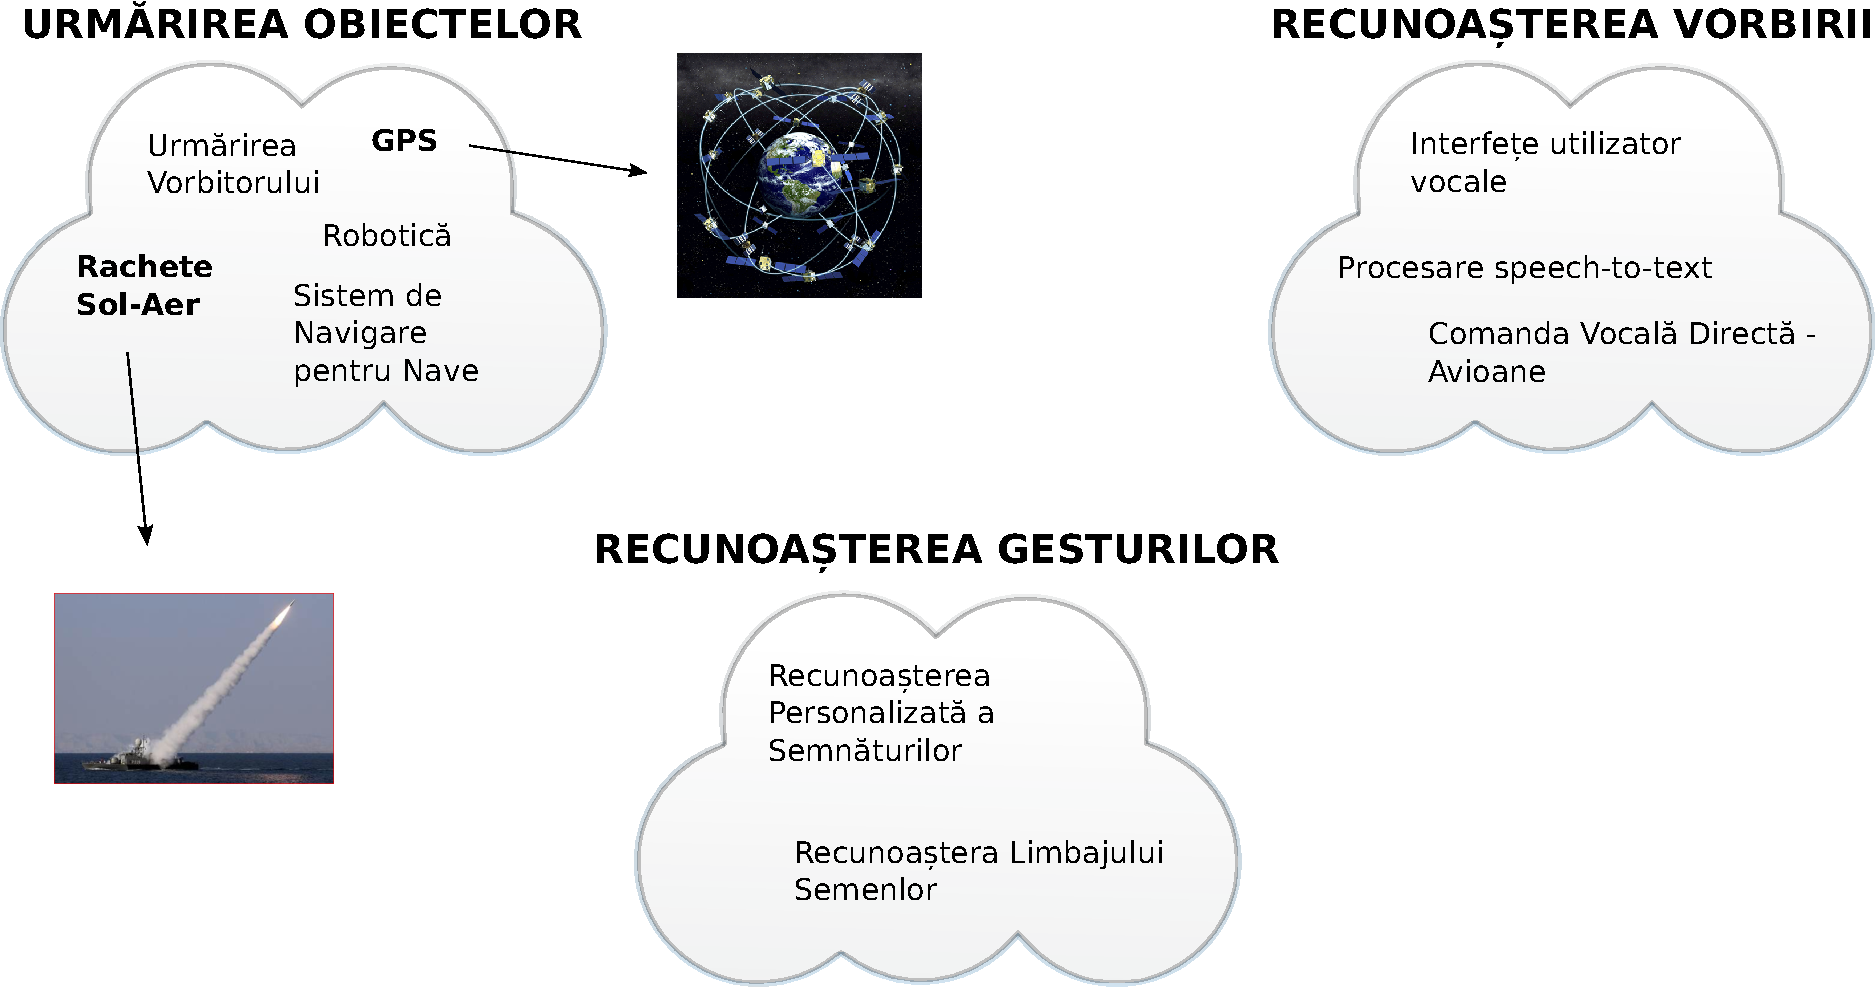
\includegraphics[width=\textwidth]{graphics/hmm-intro/time_series_problems_1_3.pdf}
  	\footnote{Sursa imaginii: http://www.hapblog.com/2012/01/iran-navy-tests-surface-to-air-missile.html}
  }
  \only<4>{
  	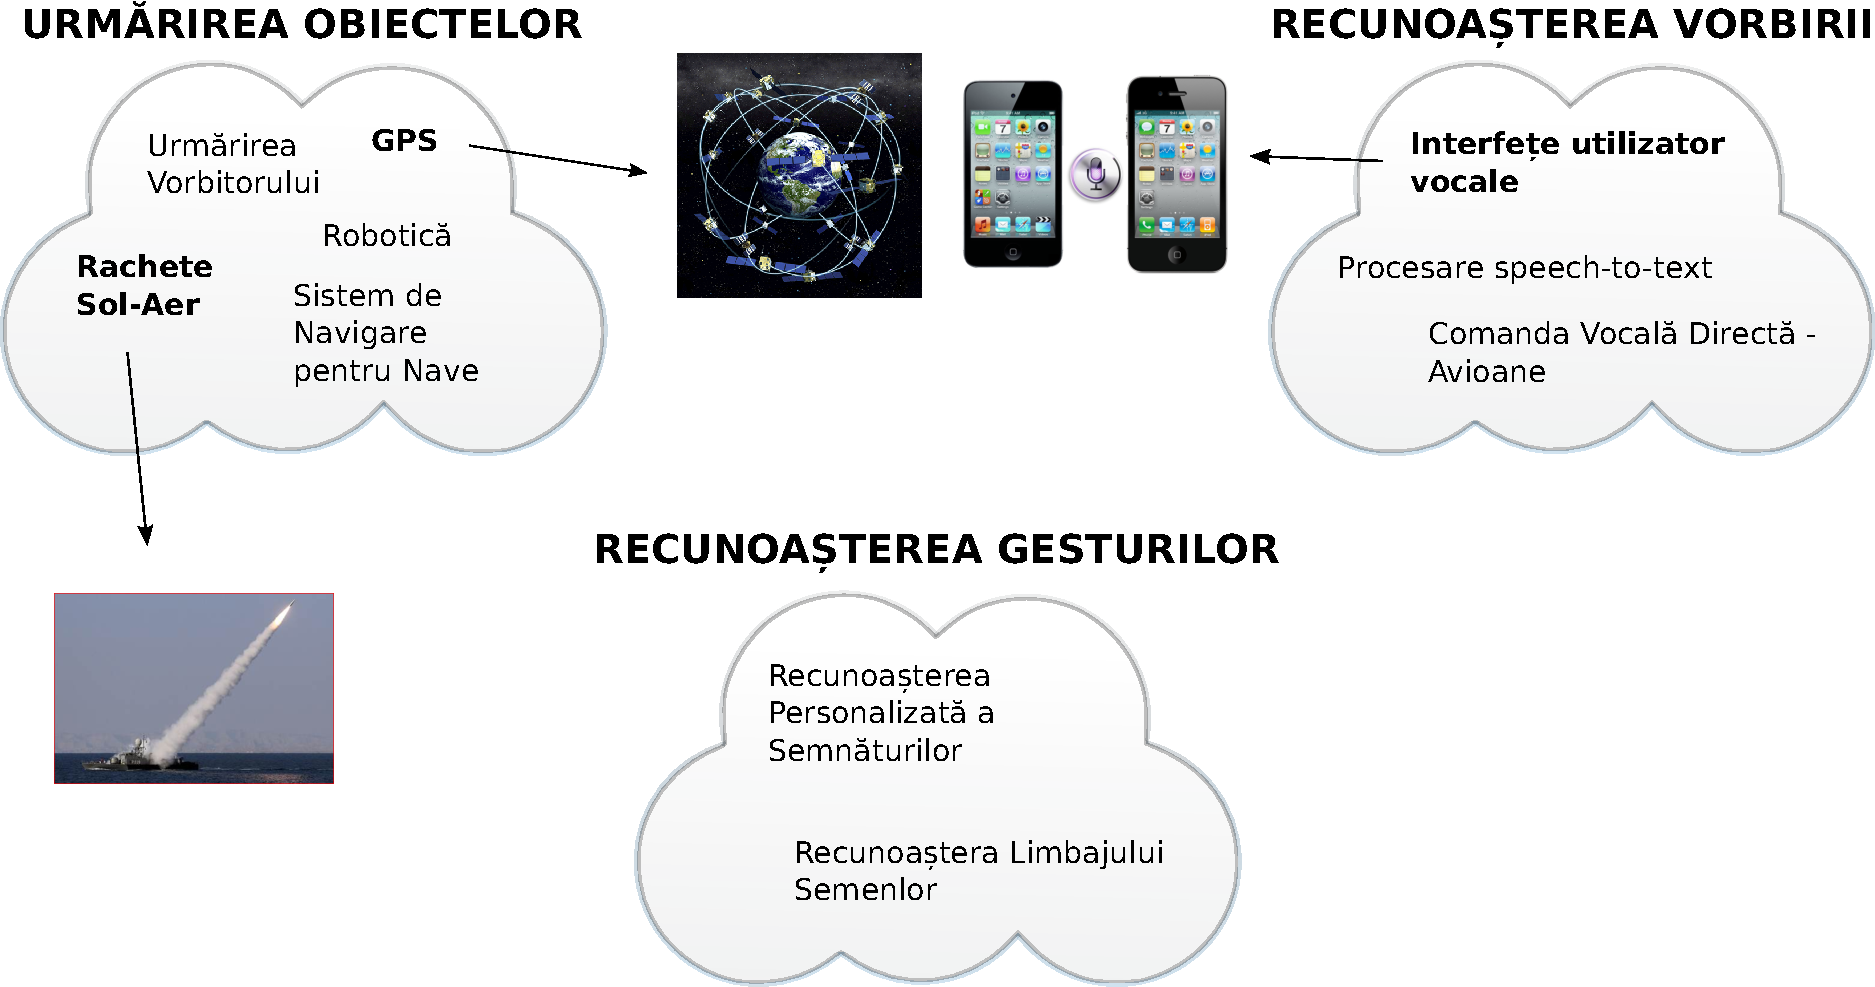
\includegraphics[width=\textwidth]{graphics/hmm-intro/time_series_problems_1_4.pdf}
  	\footnote{Sursa imaginii: http://www.redmondpie.com/}
  }
  \only<5>{
  	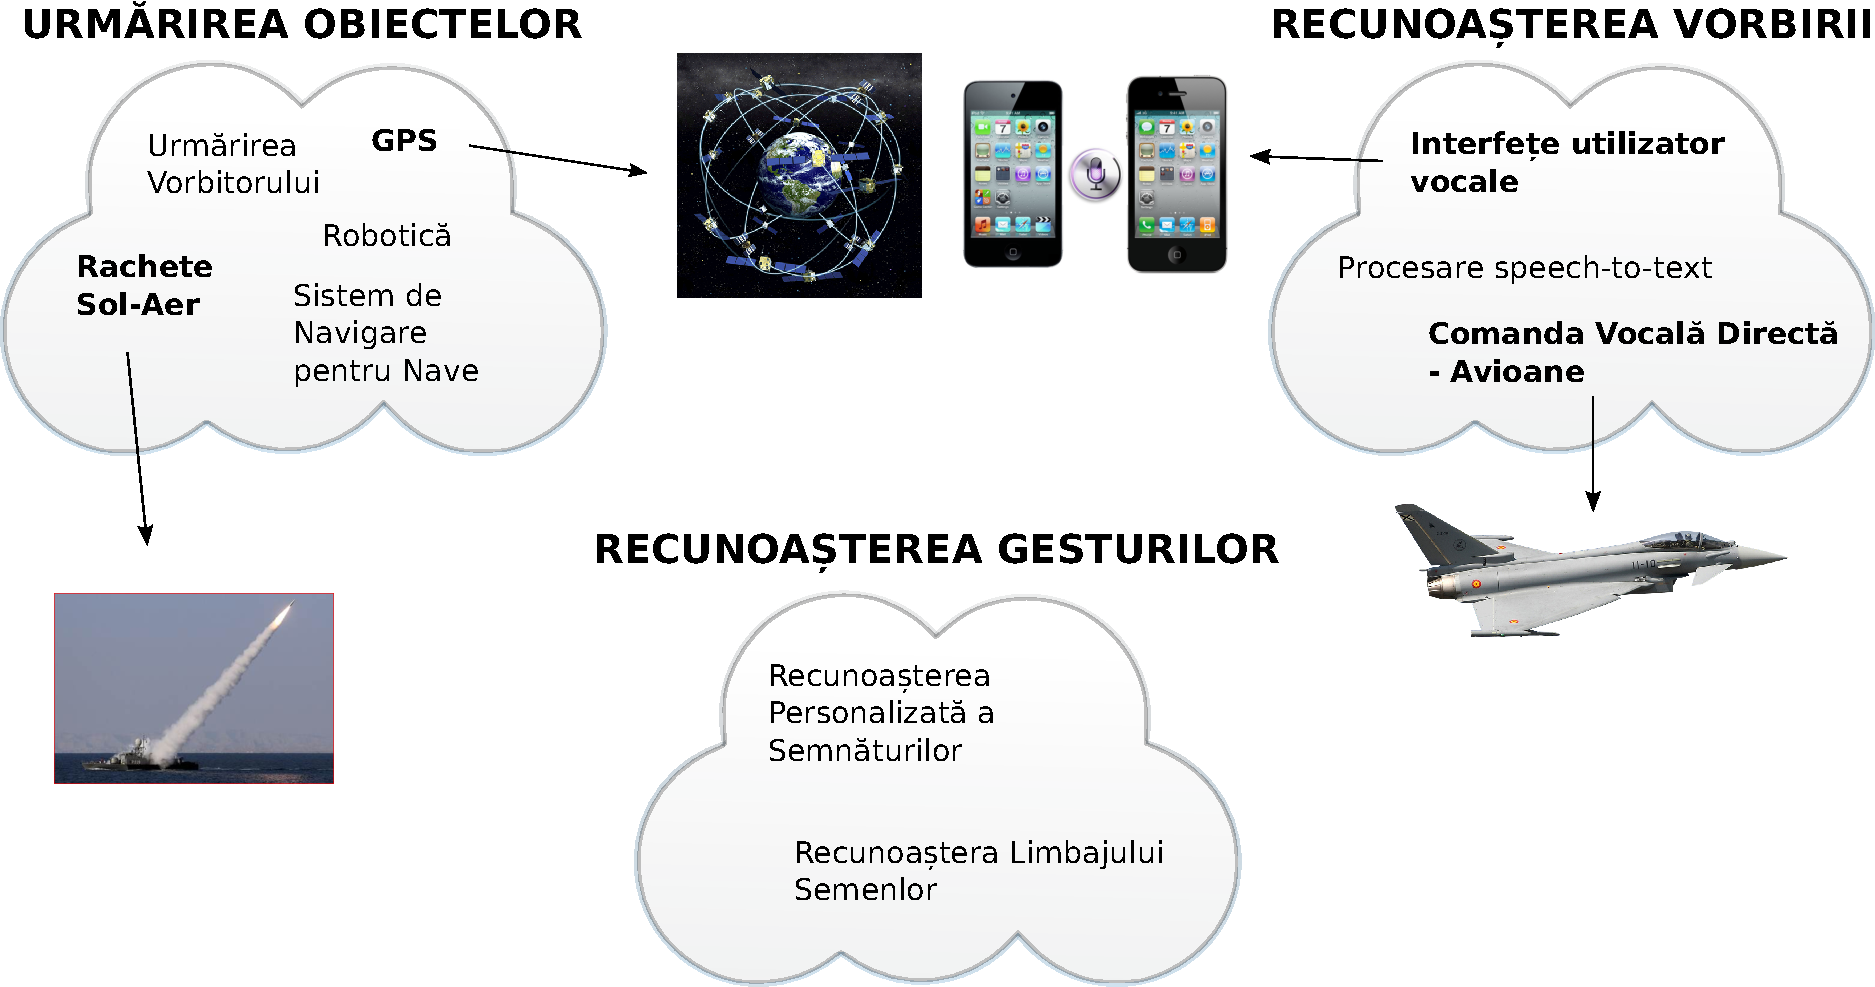
\includegraphics[width=\textwidth]{graphics/hmm-intro/time_series_problems_1_5.pdf}
  	\footnote{Sursa imaginii: http://desura.com}
  }
  \only<6>{
  	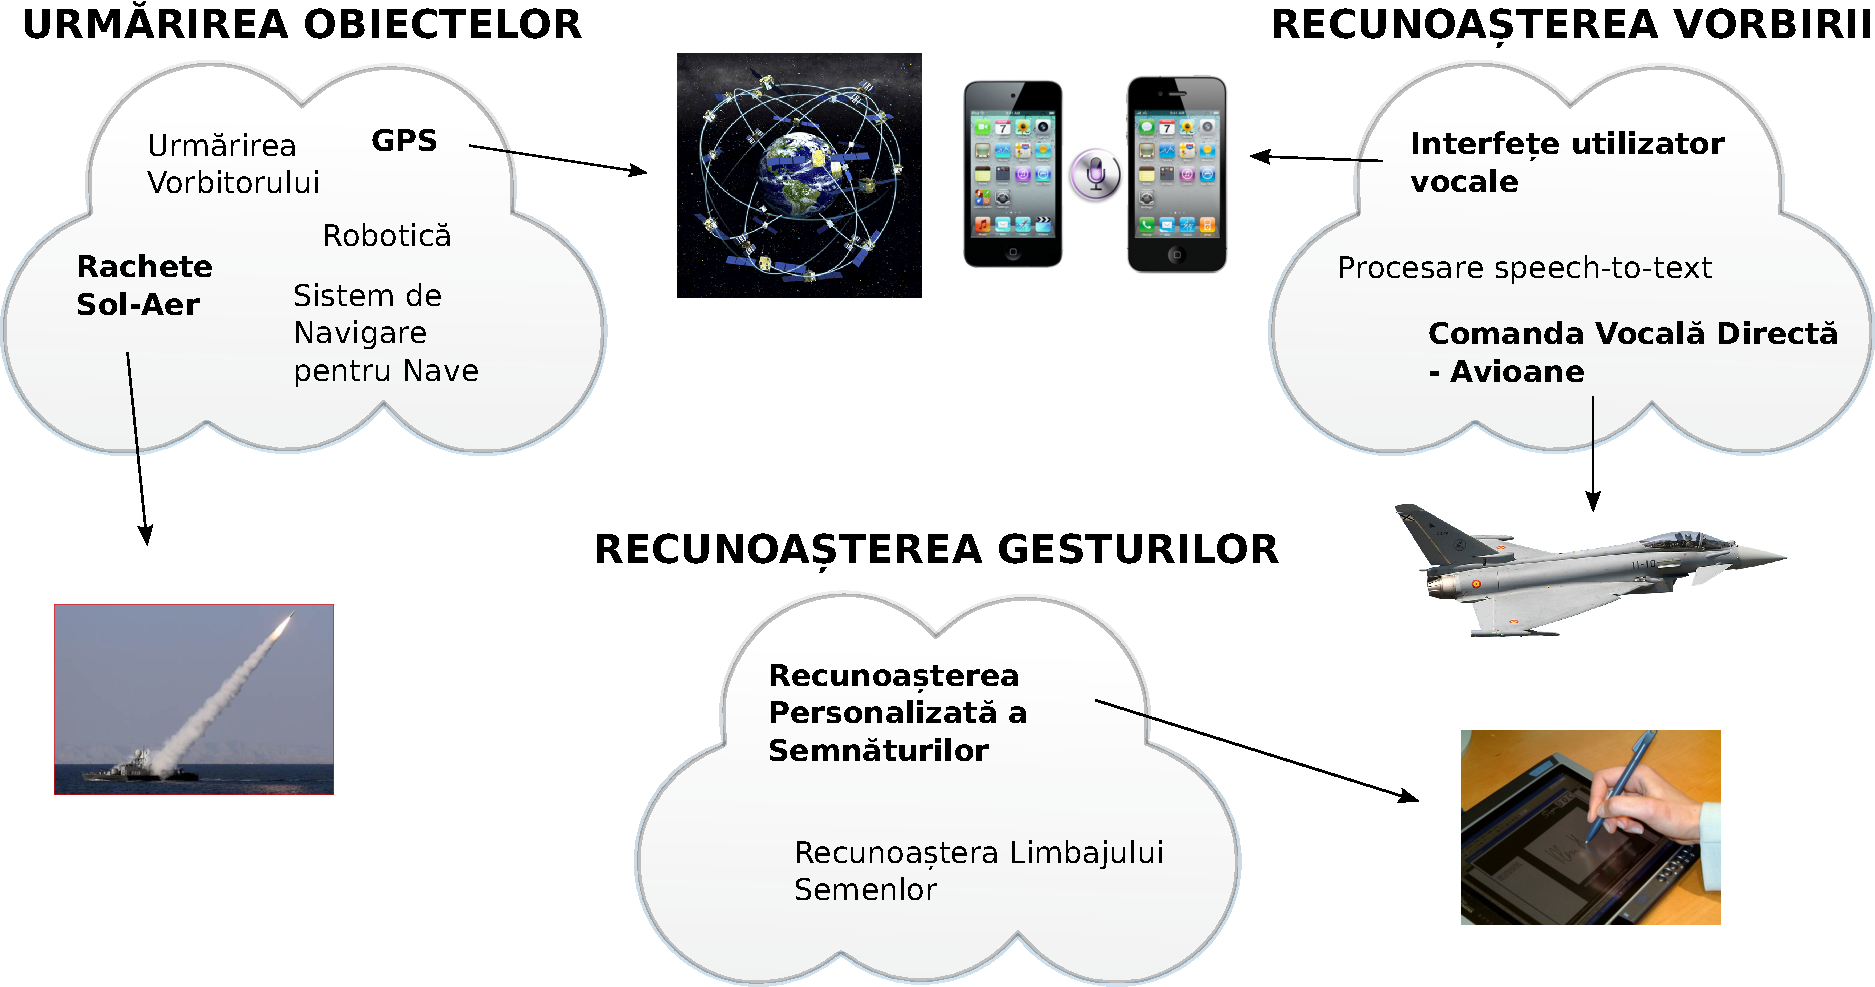
\includegraphics[width=\textwidth]{graphics/hmm-intro/time_series_problems_1_6.pdf}
  	\footnote{Sursa imaginii:  http://www.softpro.de}
  }
  
\end{frame}

\begin{frame}
  \frametitle{Probleme cu Secvențe Temporale (II)}
  \only<1>{
  	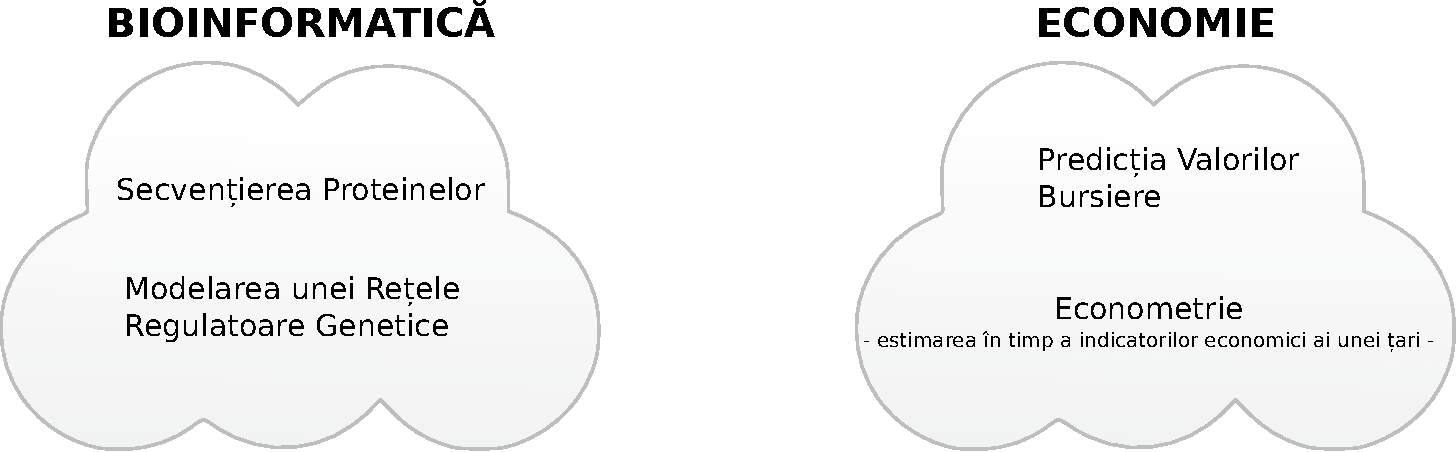
\includegraphics[width=\textwidth]{graphics/hmm-intro/time_series_problems_2.pdf}
  }
  \only<2>{
  	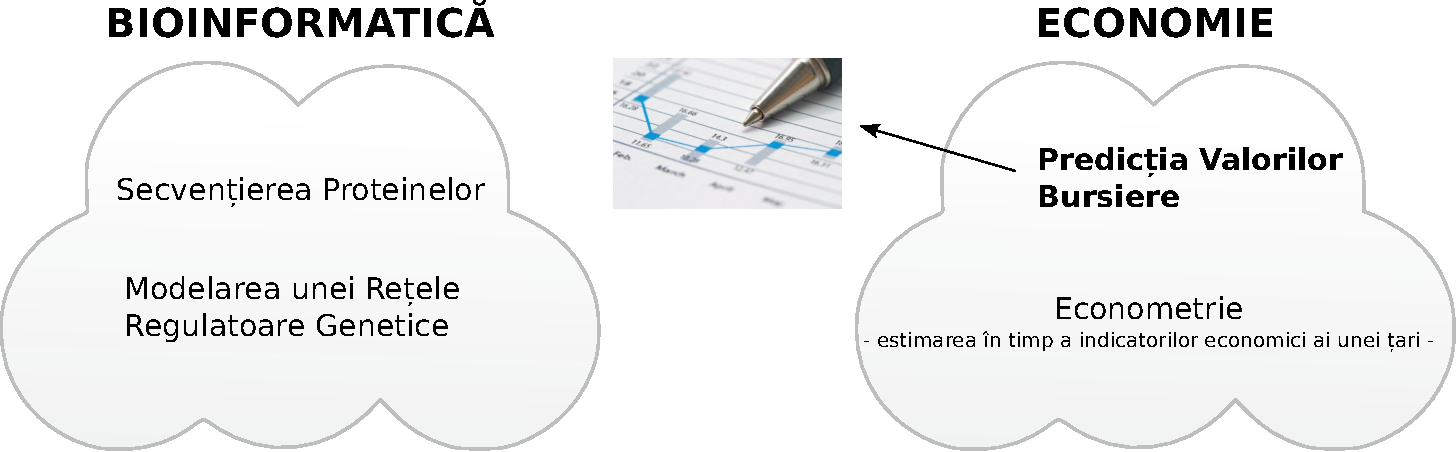
\includegraphics[width=\textwidth]{graphics/hmm-intro/time_series_problems_2_2.pdf}
  	\footnote{Sursa imaginii:  http://www.econ.ucsb.edu/~doug/}
  }
\end{frame}


% descrierea a ceea ce inseamna Probabilistic Reasoning over Time (capitol 15.2 AI a modern approach)
% 	- states and observations
\begin{frame}[t]
  \frametitle{Raționament Probabilistic Temporal - Modele}
	
	Să ne gândim la unele din problemele anterioare ...	
	\vspace*{0.5em}
	\pause	
	
	Cum modelăm astfel de situații dinamice? 
	\vspace*{0.5em}
	\pause	
	
	\textbf{Stări și Observații}
	\begin{itemize}
		\item Procesul de schimbare este văzut ca o serie de \alert{snapshot-uri}
		\item Fiecare snapshot conține un set de variabile aleatoare
    	\begin{itemize}
			\item $\mathbf{O}_t$ - setul tuturor variabilelor de măsurare (\alert{\emph{observabile}}) la momentul \emph{t}
			\item $\mathbf{Q}_t$ - setul tuturor variabilelor de stare (\alert{\emph{neobservabile / ascunse}}) la momentul \emph{t}	    	
		\end{itemize}
	\end{itemize}
	
	\begin{figure}
		\centering
		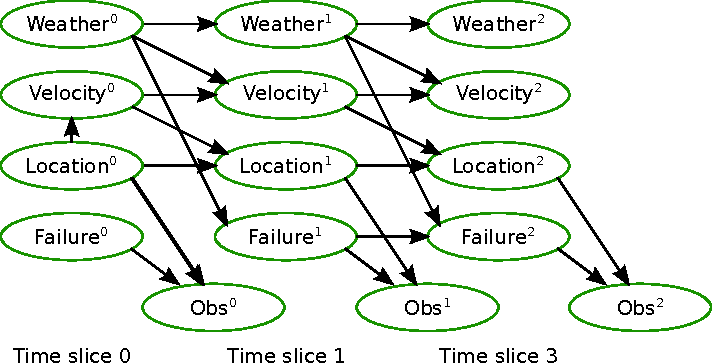
\includegraphics[height=0.3\textheight]{graphics/hmm-intro/dbn-vehicle/unrolled.pdf} 
  		\caption{\tiny{Exemplu: problemă de localizare a unui vehicul \citep{KollerFriedman09}}}
  		\label{fig:unrolled-states-observations}
  	\end{figure}
\end{frame}

%	- stationary process, Markov assumption, Sensor model
\begin{frame}[t]
  \frametitle{Raționament Probabilistic Temporal - Presupuneri}
	Să ne gândim la unele din problemele anterioare ...	
	\vspace*{0.5em}
	\pause	
	
	Ce \alert{presupuneri} (la o adică) facem?
	\pause	
	
	\begin{block}{Proces staționar}
		Procesul de schimbare este guvernat de legi care \alert{nu se schimba in timp}.\\
		\alert{Urmare:} trebuie sa specificăm relațiile între variabile doar pentru un snapshot \emph{reprezentativ}.	
	\end{block}
	\pause	
	
	\begin{block}{Presupunerea Markov}
		Starea curentă a unui proces de schimbare depinde doar de o \alert{istorie finită} de stări anterioare.\\
		\alert{Urmare:} avem un număr \alert{limitat} de ``parinți'' pentru variabilele din fiecare snapshot.
	\end{block}
  
\end{frame}

%	- inference in temporal models
%		- filtering
%		- prediction
%		- smoothing (hindsight)
%		- most likely explanation
%		- model learning
\begin{frame}
  \frametitle{Raționament Probabilistic Temporal - Inferență}
	Care sunt principalele inferențe ce se doresc făcute?	
	\pause	
	
	\begin{block}{Filtrare (monitorizare)}
		Sarcina de a calcula \alert{starea de fapt} - distribuția posterioară de probabilitate a 
		\alert{stării curente}, date fiind toate observațiile de până acum.
	\end{block}
	\pause
	
	\begin{block}{Evaluare}
		Sarcina de a calcula \alert{probabilitatea (likelihood)} a observațiilor făcute până în prezent.
	\end{block}  
\end{frame}

\begin{frame}
  \frametitle{Raționament Probabilistic Temporal - Inferență}
	\begin{block}{Predicție}
		Sarcina de a calcula distribuția posterioară de probabilitate peste o \alert{stare viitoare}, 
		date fiind toate observațiile de până acum.
	\end{block}
	\pause
	
	\begin{block}{Netezire (hindsight)}
		Sarcina de a calcula distribuția posterioară de probabilitate peste o \alert{stare anterioară}, 
		date fiind toate observațiile de până acum.\\
		Furnizează o estimare mai buna asupra stării respective, decât a fost posibil la momentul respectiv.
	\end{block}
\end{frame}

\begin{frame}
  \frametitle{Raționament Probabilistic Temporal - Inferență}
	\begin{block}{Cea mai probabilă explicație}
		Dându-se o \emph{secvență de observații}, se cere găsirea \alert{celei mai probabile secvenței de stări}
		care a generat acele observații.
	\end{block}
	\pause
	
	\begin{block}{Învățare}
		Dându-se \emph{un set de secvențe de observații}, găsește o metodă de a învăța \alert{modelele} de
		\alert{tranziție} și \alert{senzoriale / de măsurare} pe baza acelor observații.
	\end{block}
\end{frame}

\begin{frame}[t]
    \frametitle{Raționament Probabilistic Temporal - Metode Cunoscute}
    
  	\begin{block}{Rețele Bayesiene Dinamice (RBD)}
  		O RBD este o rețea Bayesiană ce reprezintă un model temporal de probabilitate.
  	\end{block}
  	
  	\begin{figure}
  		\centering
		\begin{subfigure}[b]{0.15\textwidth}
			\centering
  			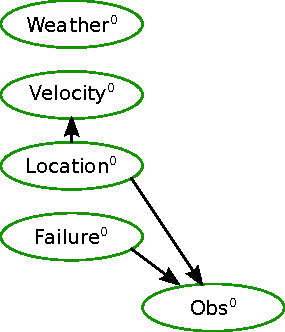
\includegraphics[width=\textwidth]{graphics/hmm-intro/dbn-vehicle/zero.pdf}
  			\caption{\tiny{Rețeaua Bayesiană în două snapshot-uri}}
  			\label{fig:2TBN}
  		\end{subfigure}
  		\begin{subfigure}[b]{0.30\textwidth}
			\centering
			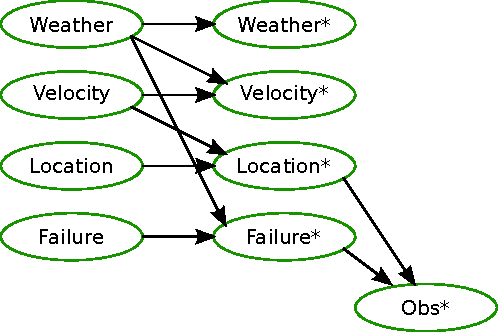
\includegraphics[width=\textwidth]{graphics/hmm-intro/dbn-vehicle/transition.pdf}
  			\caption{\tiny{Rețeaua la momentul 0}}
  			\label{fig:zeroDBN}
  		\end{subfigure}
  		\begin{subfigure}[b]{0.35\textwidth}
			\centering
			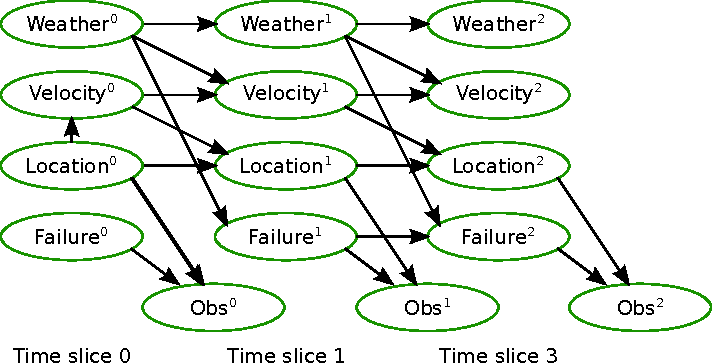
\includegraphics[width=\textwidth]{graphics/hmm-intro/dbn-vehicle/unrolled.pdf} 
  			\caption{\tiny{RBD desfășurată pe 3 momente de timp}}
  			\label{fig:unrolledDBN}
  		\end{subfigure}
  		\caption{\tiny{RBD simplificată pentru monitorizarea unui vehicul \citep{KollerFriedman09}}}
  		\label{fig:DBN}
  	\end{figure}
  	
  	\small{Aplicată în probleme precum: urmărirea obiectelor, recunoașterea activității umane, secvențierea proteinelor, etc.}
\end{frame}


\begin{frame}[t]
    \frametitle{Raționament Probabilistic Temporal - Metode Cunoscute}
  
  \begin{block}{Filtre Kalman (Sistem Dinamice Lineare)}
	Un model temporal având una sau mai multe variabile care evoluează linear în timp, la care se adaugă 
	\alert{zgomot Gaussian}.
  \end{block}
  
  \begin{columns}[T]
  	\column{0.4\textwidth}
  	\begin{figure}
  		\centering
  		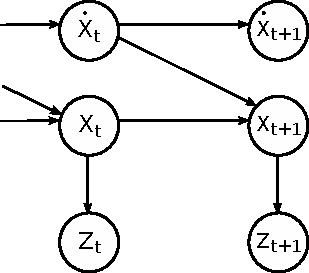
\includegraphics[height=0.35\textheight]{graphics/hmm-intro/kalman/kalman_filter_simple.pdf}
  		\caption{\tiny{Structura unei RB pentru un sistem linear dinamic cu variabile de poziție $X_t$, 
  		viteză $\dot{X}_t$, și măsurare a poziției $Z_t$}}
  	\end{figure}
	  
  	\column{0.6\textwidth}
  	\begin{itemize}
  		\item \footnotesize{Poate fi văzut ca o RBD în care toate variabilele sunt continue, iar dependențele sunt 
  		linear gaussiane.}
  		\item \footnotesize{Aplicații multiple în \textbf{urmărirea obiectelor}}
  	\end{itemize}
  \end{columns}
  
\end{frame}

\begin{frame}[t]
    \frametitle{Raționament Probabilistic Temporal - Metode Cunoscute}
  
  \begin{block}{Modele Markov Ascunse (MMA)}
	Un MMA (HMM) este un model probabilistic temporal în care \emph{starea} procesului de schimbare este descrisă
	de \alert{o singură variabilă aleatoare discretă}.
	Valorile posibile ale variabilei reprezintă stările posibile ale lumii modelate.
  \end{block}
  
  \vspace*{1em}
  
  Utilizat cu succes in aplicații precum:
  \begin{itemize}
  	\item Recunoasțerea Scrisului
  	\item Recunoasțerea Gesturilor
  	\item Recunoasțerea Vorbirii
  	\item Determinarea Parților de Vorbire (Part-of-Speech Tagging)
  	\item Secvențiere ADN
  \end{itemize}
\end{frame}



\section{Teoria MMA}
\label{sec:theory}

\subsection{Cele Trei Probleme ale MMA}
\label{sec:three-problmes}

%% alejandro
\section{Theory of HMMs}
\label{sec:theory}

\subsection{The 3 things you want from an HMM}
\label{sec:problems}

\begin{frame}
  
  The 3 fundamental problems \parencite{rabiner1989tutorial}
  \begin{itemize}
  	\item Particularization of temporal inference problems to the HMM case
  	\item The restricted structure of the HMM allows for elegant implementations of all the basic algorithms
  \end{itemize}
  \pause

  \begin{block}{Evaluation Problem}
    Given a model and a sequence of observations, how do we compute the probability that the \alert{observed 
    sequence} was produced by the model?
  \end{block}
  \pause
  \begin{block}{Best Explanation of Observations Problem}
    Given a model and a sequence of observations how do we choose a corresponding sequence of \alert{states} which 
    \emph{gives meaning} to the observations? How do we \emph{uncover} the hidden part of the model?
  \end{block}
  \pause
  \begin{block}{Model Estimation (Training) Problem}
    Given some observed sequences, how do we adjust the \alert{parameters} of an HMM model that best tries to explain 
    the observations? 
    
  \end{block}

\end{frame}


\subsection{Mathematical Foundations for HMMs}
\label{sec:math}



\begin{frame}
  \frametitle{An example problem: Emotional states}
  \begin{columns}[T]
    \column{0.58\textwidth}
    \only<1>{\framebox{
\includegraphics[width=\textwidth]{all/hmm-final-m.pdf}}}
    \only<2>{\framebox{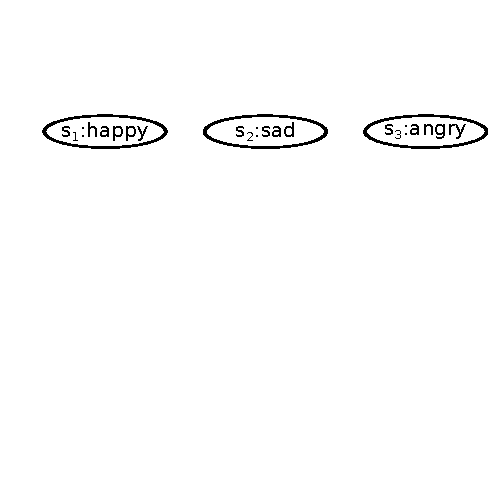
\includegraphics[width=\textwidth]{all/hmm-final-n.pdf}}}
    \only<3>{\framebox{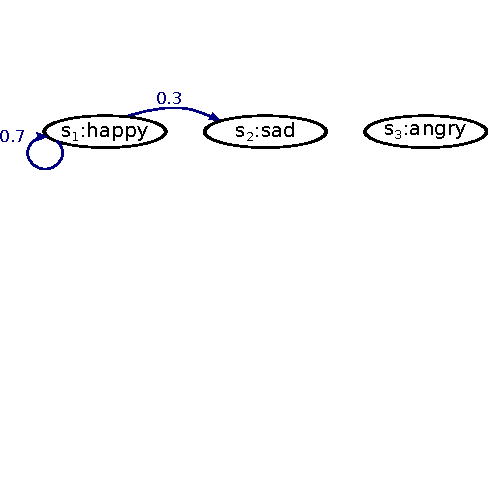
\includegraphics[width=\textwidth]{all/hmm-final-o.pdf}}}
    \only<4>{\framebox{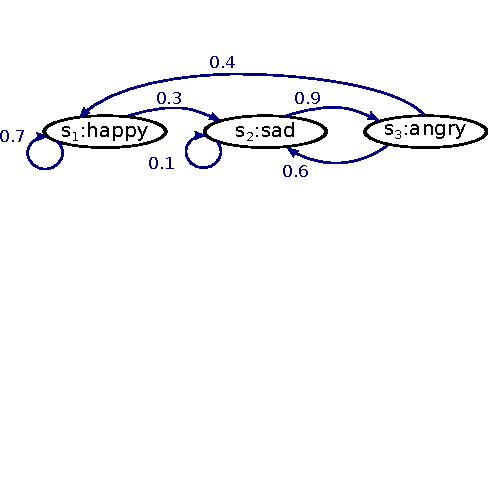
\includegraphics[width=\textwidth]{all/hmm-final-q.pdf}}}
    \only<5>{\framebox{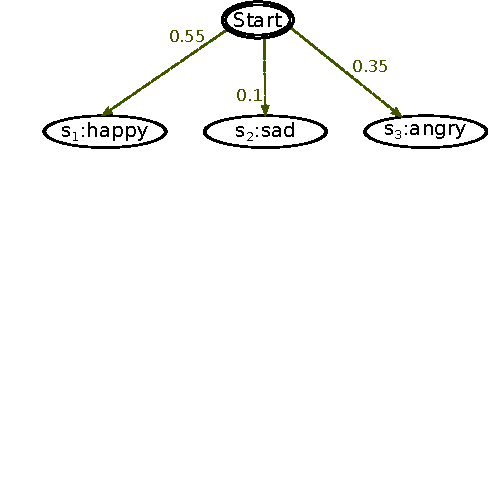
\includegraphics[width=\textwidth]{all/hmm-final-r.pdf}}}
    \only<6>{\framebox{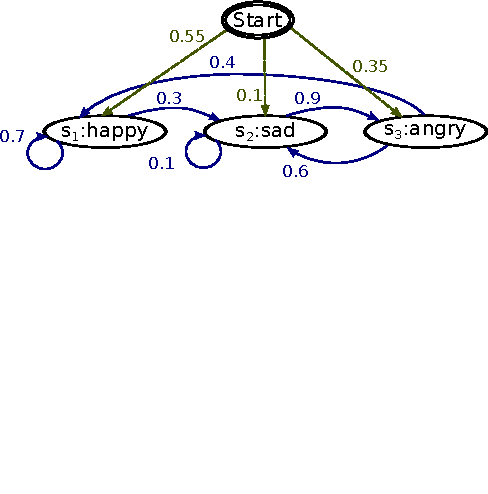
\includegraphics[width=\textwidth]{all/hmm-final-s.pdf}}}
    \only<7>{\framebox{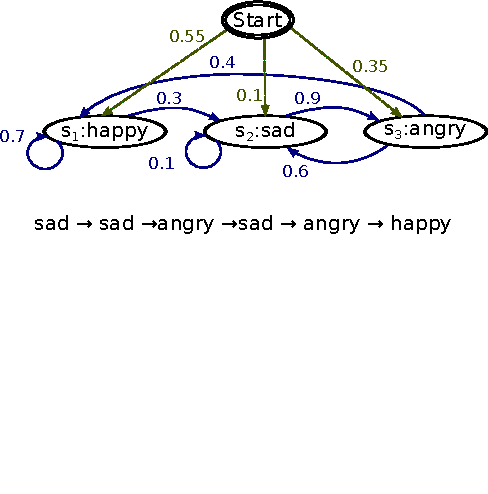
\includegraphics[width=\textwidth]{all/hmm-final-t.pdf}}}
    \only<8>{\framebox{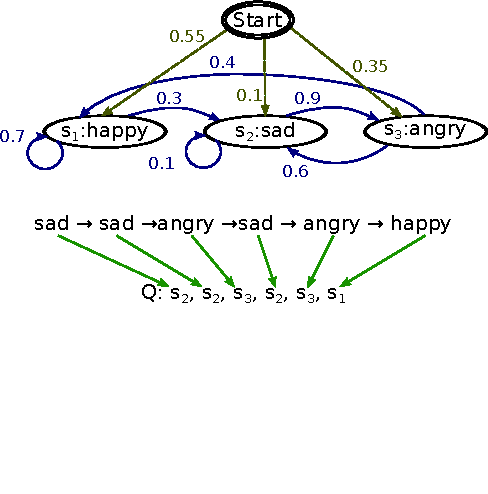
\includegraphics[width=\textwidth]{all/hmm-final-u.pdf}}}
    \only<9>{\framebox{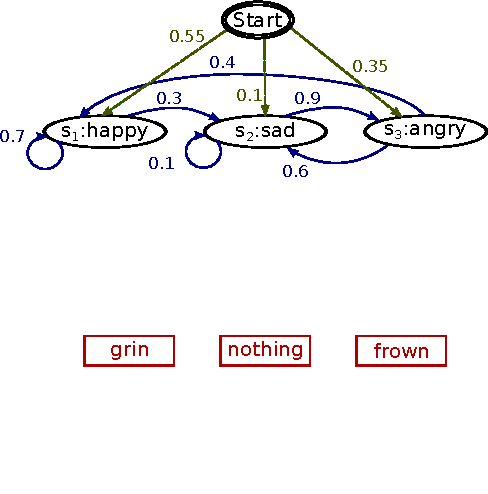
\includegraphics[width=\textwidth]{all/hmm-final-v.pdf}}}
    \only<10>{\framebox{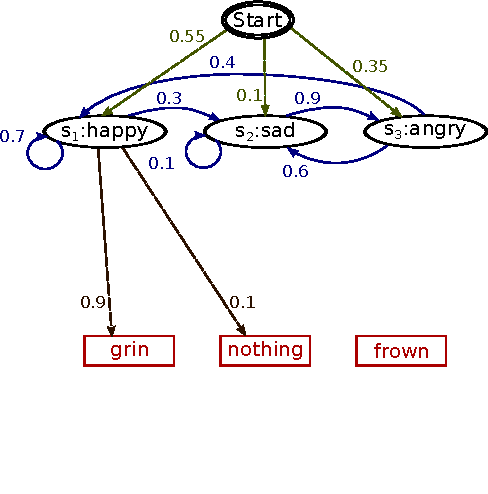
\includegraphics[width=\textwidth]{all/hmm-final-v2.pdf}}}
    \only<11-12>{\framebox{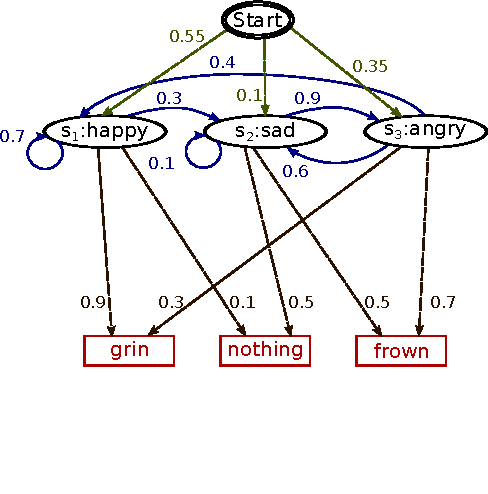
\includegraphics[width=\textwidth]{all/hmm-final-w.pdf}}}
    \only<13>{\framebox{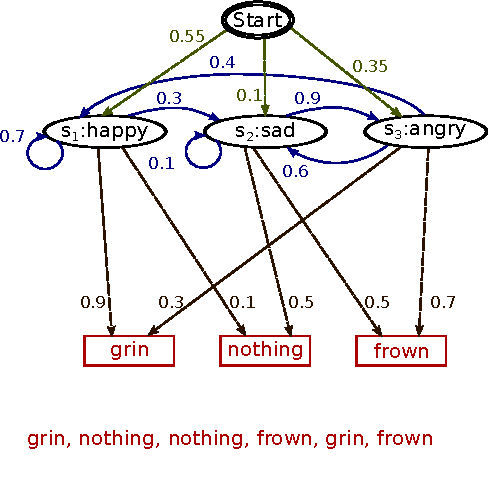
\includegraphics[width=\textwidth]{all/hmm-final-x.pdf}}}
    \only<14>{\framebox{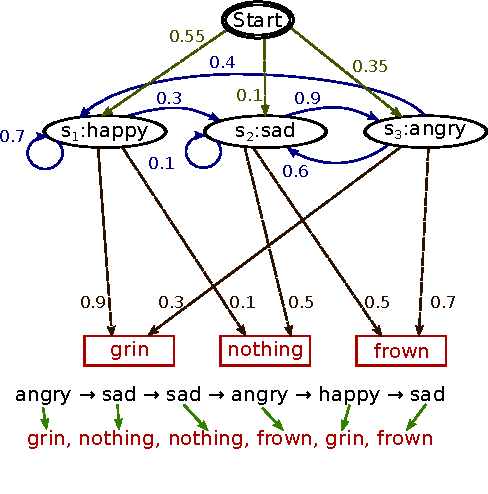
\includegraphics[width=\textwidth]{all/hmm-final-y.pdf}}}
    \only<15>{\framebox{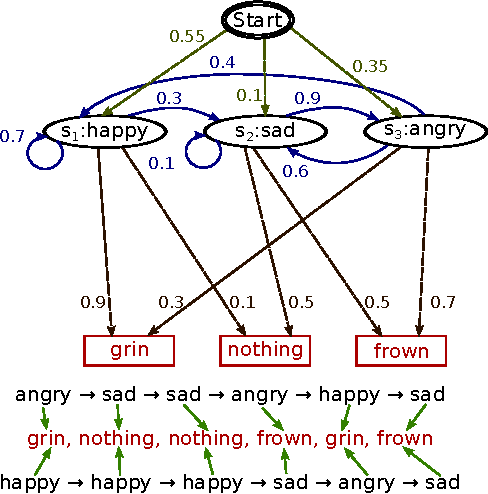
\includegraphics[width=\textwidth]{all/hmm-final-z.pdf}}}
    \only<16> {
      \begin{itemize}
      \item Example inspired from: \\\vspace*{1em}
        \fullcite{zubek2006introduction}
      \end{itemize}

    }
    

    \column{0.4\textwidth} \only<1>{ Let's consider a simple example:
      \\ \ a robot that tracks the emotional states of a player.  }
    \only<2>{ $\mathbf{N}$ - number of states \\ \vspace*{.5em}
      $\mathbf{N}=3$ \\ \vspace*{.5em} states:
      \begin{itemize}
      \item $s_1$: happy
      \item $s_2$: sad
      \item $s_3$: angry
      \end{itemize}

    }\only<3-4> { $\mathbf{A}$ - state transition probability
      distribution \\ \vspace*{.5em} \small{ $\mathbf{A} = \lbrace
        a_{i,j} \rbrace, \: 1 \le i, j \le N$ \\ \vspace*{.5em}
        $a_{i,j} = P(q_{t+1}=s_j \vert q_t = s_i)$
        \begin{itemize}
        \item $a_{\mathbf{1},1} = 0.7$
        \item $a_{\mathbf{1},2} = 0.3$
        \item $a_{\mathbf{1},3} = 0$
        \end{itemize}
        $\displaystyle\sum_{j=1}^{N}a_{i,j}=1, \quad 1 \le i \le N$ }
      \visible<4-> { $\mathbf{A} = \bordermatrix{~ & s_1 & s_2 & s_3
          \cr s_1 & 0.7 & 0.3 & 0 \cr s_2 & 0 & 0.9 & 0.1 \cr s_3 &
          0.4 & 0.6 & 0 \cr}$ }

    }
    
    \only<5>{ $\mathbf{\Pi}$ - initial state distribution \\
      \vspace*{0.5em} $\mathbf{\Pi} = \lbrace \pi_i \rbrace,\quad 1
      \le i \le N$ \\ \vspace*{0.5em} $\pi_i = P(q_1 = s_i)$ \\
      \vspace*{0.5em}
      
      $ \mathbf{\Pi} = \bordermatrix{ ~ & s_1 & s_2 & s_3 \cr ~ & 0.35
        & 0.1 & 0.55 \cr} $ }
    
    \only<6-8>{ $A = \bordermatrix{~ & s_1 & s_2 & s_3 \cr s_1 & 0.7 &
        0.3 & 0 \cr s_2 & 0 & 0.9 & 0.1 \cr s_3 & 0.4 & 0.6 & 0 \cr}$
      \\ \vspace*{0.25em} $\Pi = \bordermatrix{ ~ & s_1 & s_2 & s_3
        \cr ~ & 0.35 & 0.1 & 0.55 \cr}$ \\ \vspace*{0.25em}
      \visible<8> { $Q = [ q_1 q_2 \cdots q_T ]$ \small{
          \begin{equation*}
            \begin{split}
              P(Q & \vert A,\Pi)= \\ & = \pi_{q_1}a_{q_1,q_2}\cdots
              a_{q_{T-1},q_T}
            \end{split}
          \end{equation*}
          \begin{equation*}
            \begin{split}
              P(s_2,s_2,s_3,s_2,s_3,s_1\vert A,\Pi) = \\
              = \pi_2 \cdot a_{2,2} \cdot a_{2,3} \cdot a_{3,2} \cdot a_{2,3} \cdot a_{3,1} \\
              = \scriptstyle{0.1 \cdot 0.3 \cdot 0.1 \cdot 0.9 \cdot 0.6 \cdot 0.9 \cdot 0.4} \\
              = \scriptstyle{0.0005832}
            \end{split}
          \end{equation*}
        } }}

    \only<9>{ $\mathbf{M}$ - number of distinct observable values \\
      \vspace*{.5em} $\mathbf{M}=3$ \\ \vspace*{.5em} values:
      \begin{itemize}
      \item $v_1$: grin
      \item $v_2$: nothing
      \item $v_3$: frown
      \end{itemize}
    }

    \only<10-11> { $\mathbf{B}$ - observation values probability
      distribution \\ \vspace*{.5em} \small{ $\mathbf{B} = \lbrace
        b_{j,k} \rbrace \: \scriptstyle{1 \le j \le N, 1 \le k, \le
          M}$
        \begin{equation*}
          \begin{split}
            b_{j,k} & =b_{j}(v_k) \\
            & =P(o_t = v_k \vert q_t = s_j)
          \end{split}
        \end{equation*}
        \vspace*{-1.5em} \scriptsize{
          \begin{itemize}
          \item $b_{\mathbf{1},1} = b_{\mathbf{1}}(grin) = 0.9$
          \item $b_{\mathbf{1},2} = b_{\mathbf{1}}(nothing) = 0.1$
          \item $b_{\mathbf{1},3} = b_{\mathbf{1}}(frown) = 0$
          \end{itemize}}
        $\displaystyle\sum_{k=1}^{M}b_{j,k}=1, \quad 1 \le j \le N$\\
      }\visible<11> { $\mathbf{B} = \bordermatrix{ ~ & grin & notg &
          frown \cr s_1 & 0.9 & 0.1 & 0 \cr s_2 & 0 & 0.5 & 0.5 \cr
          s_3 & 0.3 & 0 & 0.7 \cr }$ } }
    
    \only<12>{ $\mathbf{\lambda}$ - parameters of the model \\
      \vspace*{.5em} $\lambda = (A, B, \Pi)$ \\ \vspace*{2em} $A$ -
      state transition probability distribution \\ \vspace*{.5em} $B$
      - observation values probability distribution \\ \vspace*{.5em}
      $\Pi$ - initial state distribution }
    
    \only<13-15>{ $\mathbf{O}$ - observation sequence \\ \vspace*{1em}
      $\mathbf{T}$ - length of observation sequence \\ \vspace*{1em}
      $O = [ o_1 o_2 \cdots o_T ]$ }

    
  \end{columns}
\end{frame}


\begin{frame}
  \frametitle{Restating the three fundamental HMM Problems}
  \begin{block}{Evaluation Problem}
    Given a model and a sequence of observations, how do we compute
    the probability that the \alert{observed sequence} was produced by
    the model?
  \end{block}
  \pause
  \begin{equation}
    P(O \vert Q, \lambda) = \displaystyle\prod_{t=1}^{T} P(o_t \vert
    q_t, \lambda)= \displaystyle\prod_{t=1}^{T} b_{q_t}(o_t) =
    b_{q_1}(o_1) \cdot \ldots \cdot b_{q_T}(o_T)
    \label{eq:pql}
  \end{equation}\pause
  \begin{equation}
    P(Q | \lambda) = \pi_{q_1}\displaystyle\prod_{t=2}^{T}
    a_{q_{t-1},q_t} = \pi_{q_1} \cdot a_{q_1,q_2} \cdot a_{q_2,q_3} \cdot \ldots \cdot
    a_{q_{T-1},q_T}\label{eq:pql2}
  \end{equation}\pause
  \begin{equation}
    \begin{split}
      P(O \vert \lambda) = \displaystyle\sum_{all\;Q} P(O, Q \vert
      \lambda) & = \displaystyle\sum_{all\;Q} P(O,\vert Q, \lambda)
      \cdot P(Q, \lambda) \\
      & = \displaystyle\sum_{all\;Q} \Big( \pi_{q_1} \cdot
      b_{q_1}(o_1) \cdot \displaystyle\prod_{t=2}^{T} b_{q_t}(o_t)
      a_{q_{t-1},q_t} \Big)
    \end{split}
    \label{eq:pql3}
  \end{equation}
\end{frame}


\subsection{Notation Conventions \& Framework Description}
\label{sec:octave}

\begin{frame}
  \frametitle{Notation Conventions}

  
\end{frame}


\begin{frame}
  \frametitle{Variables in Octave}

  
\end{frame}


\subsection{Fundamente Matematice}
\label{sec:math-foundations}

%% tudor
\begin{frame}
  \frametitle{Exemplu: Urmărirea stărilor emoționale}
  \begin{columns}[T]
    \column{0.58\textwidth}
    \only<1>{\framebox{
\includegraphics[width=\textwidth]{graphics/toy-example/example-k.pdf}}}
    \only<2>{\framebox{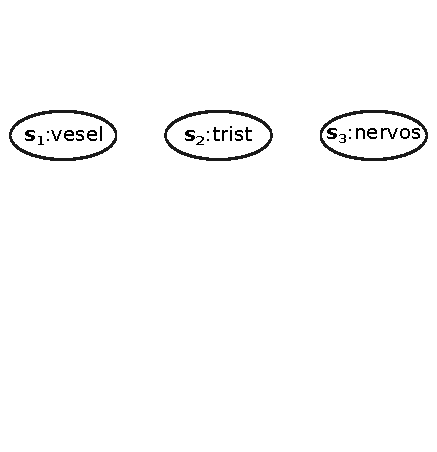
\includegraphics[width=\textwidth]{graphics/toy-example/example-l.pdf}}}
    \only<3>{\framebox{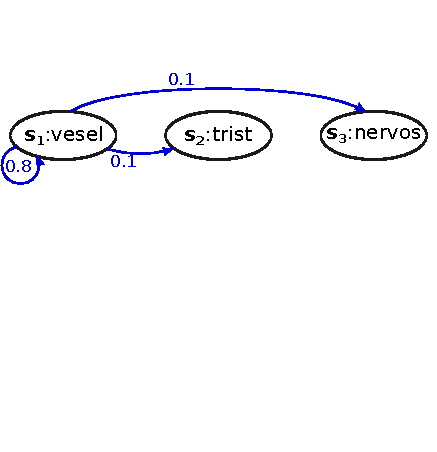
\includegraphics[width=\textwidth]{graphics/toy-example/example-m.pdf}}}
    \only<4>{\framebox{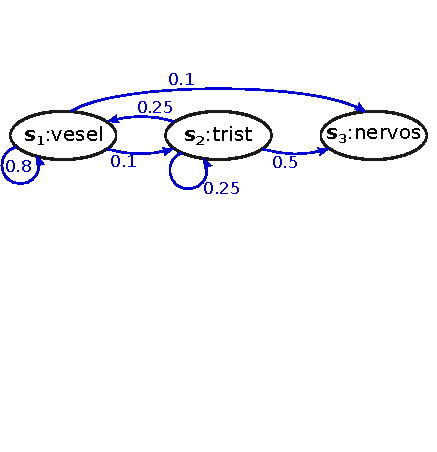
\includegraphics[width=\textwidth]{graphics/toy-example/example-n.pdf}}}
    \only<5>{\framebox{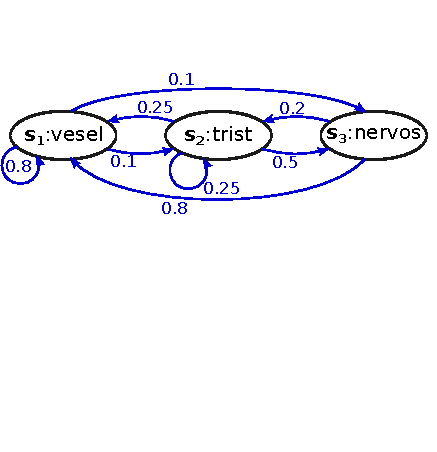
\includegraphics[width=\textwidth]{graphics/toy-example/example-o.pdf}}}
    \only<6>{\framebox{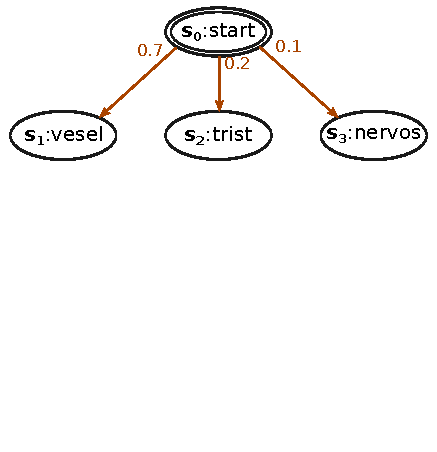
\includegraphics[width=\textwidth]{graphics/toy-example/example-p.pdf}}}
    \only<7>{\framebox{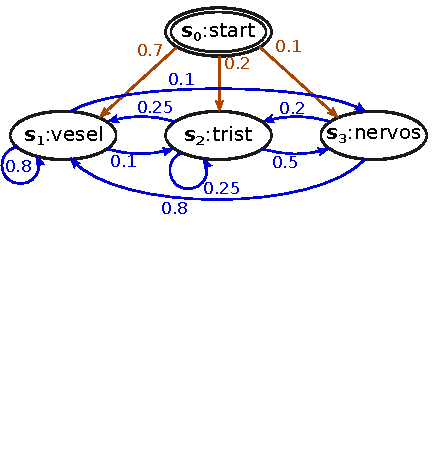
\includegraphics[width=\textwidth]{graphics/toy-example/example-q.pdf}}}
    \only<8>{\framebox{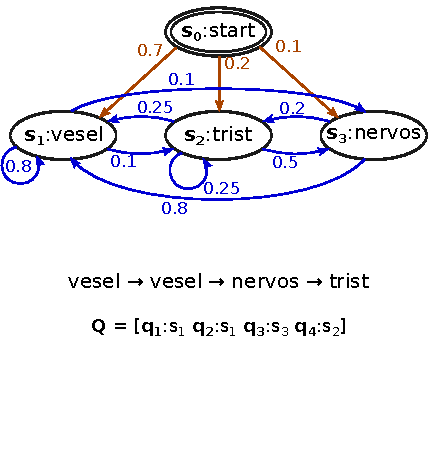
\includegraphics[width=\textwidth]{graphics/toy-example/example-r.pdf}}}
    \only<9>{\framebox{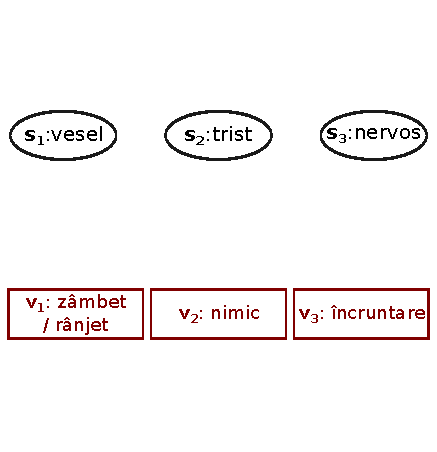
\includegraphics[width=\textwidth]{graphics/toy-example/example-s.pdf}}}
    \only<10>{\framebox{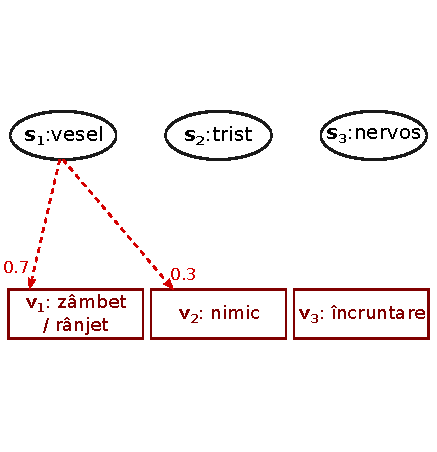
\includegraphics[width=\textwidth]{graphics/toy-example/example-t.pdf}}}
    \only<11>{\framebox{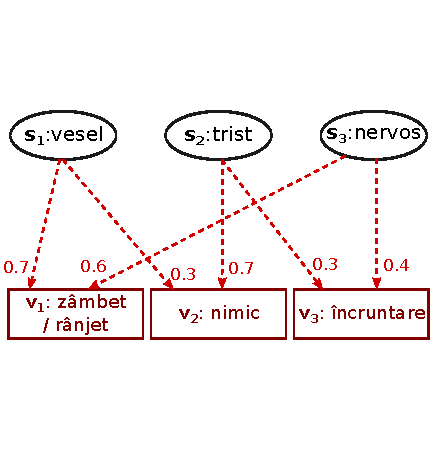
\includegraphics[width=\textwidth]{graphics/toy-example/example-u.pdf}}}
    \only<12>{\framebox{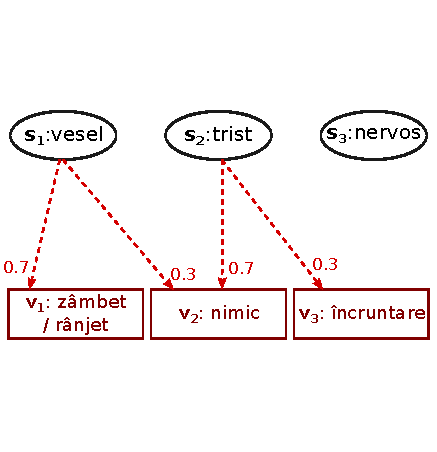
\includegraphics[width=\textwidth]{graphics/toy-example/example-v2.pdf}}}
    \only<13>{\framebox{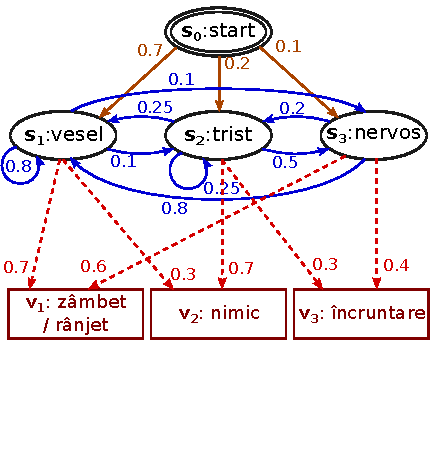
\includegraphics[width=\textwidth]{graphics/toy-example/example-v.pdf}}}
    \only<14>{\framebox{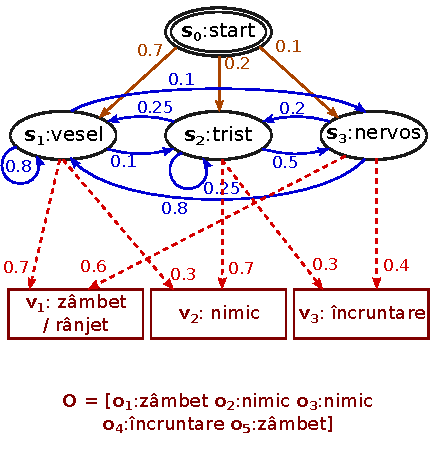
\includegraphics[width=\textwidth]{graphics/toy-example/example-w.pdf}}}
    \only<15>{\framebox{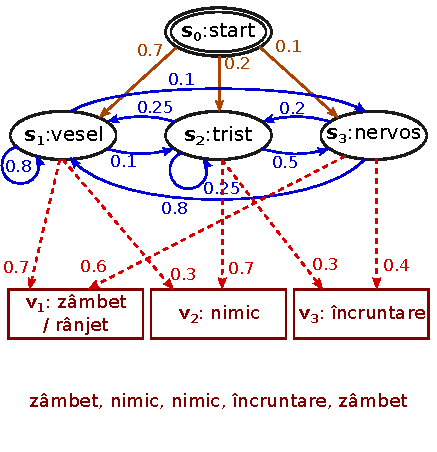
\includegraphics[width=\textwidth]{graphics/toy-example/example-x.pdf}}}
    \only<16>{\framebox{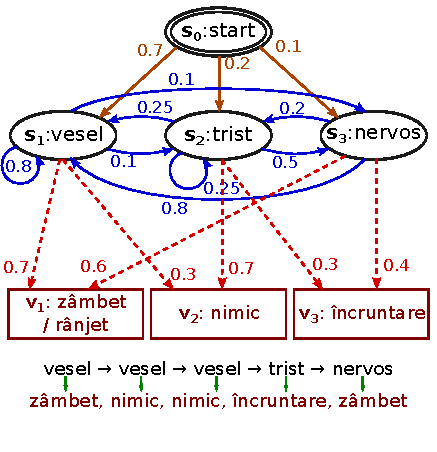
\includegraphics[width=\textwidth]{graphics/toy-example/example-y.pdf}}}
    \only<17>{\framebox{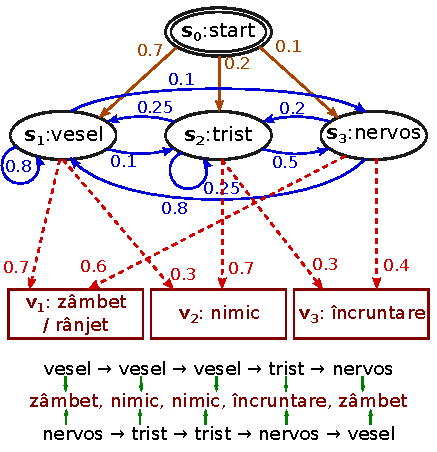
\includegraphics[width=\textwidth]{graphics/toy-example/example-z.pdf}}}
    \only<18> {
      \begin{itemize}
      \item Exemplul a fost adaptat după: \\\vspace*{1em}
        \def\newblock{} \nobibliography{}
        \bibentry{zubek2006introduction}
      \end{itemize}
      
    }
    

    \column{0.4\textwidth} \only<1>{ Să considerăm următorul exmeplu:
      \begin{itemize}
      \item un robot ce urmărește evoluția stărilor emoționale ale
        unui om
      \end{itemize}
      \vspace*{1em} Senzor:
      \begin{itemize}
      \item cameră video
      \end{itemize}
      \vspace*{1em} Să modelăm împreună această problemă definind
      componentele unui Model Markov Ascuns!  }  \only<2>{
      $\mathbf{N}$
      - numărul de stări ascunse \\ \vspace*{.5em} $\mathbf{N}=3$ \\
      \vspace*{.5em} Stări:
      \begin{itemize}
      \item $\mathbf{s_1}$: vesel
      \item $\mathbf{s_2}$: trist
      \item $\mathbf{s_3}$: nervos
      \end{itemize}

    }\only<3-5> { $\mathbf{A}$ - matricea distribuțiilor de
      probabilitate ale tranzițiilor între stări \\ \vspace*{.5em}
      \small{ $\mathbf{A} = \lbrace a_{i,j} \rbrace, \: 1 \le i, j \le
        N$ \\ \vspace*{.5em} $a_{i,j} = P(q_{t+1}=s_j \vert q_t =
        s_i)$ \\
        \horiline $\displaystyle\sum_{j=1}^{N}a_{i,j}=1, \quad 1
        \le i \le N$ } \\
      \horiline \visible<3-> { $\mathbf{A} = \bordermatrix{~ & s_1 &
          s_2 & s_3 \cr s_1 & 0.8 & 0.1 & 0.1 \cr s_2 &
          \visible<4->{0.25} & \visible<4->{0.25} & \visible<4->{0.5}
          \cr s_3 & \visible<5->{0.8} & \visible<5->{0.2} &
          \visible<5->{0} \cr}$ }
      
    }
    
    \only<6>{ $\mathbf{\Pi}$ - distribuția stării inițiale \\
      \vspace*{0.5em} $\mathbf{\Pi} = \lbrace \pi_i \rbrace,\quad 1
      \le i \le N$ \\ \vspace*{0.5em} $\pi_i = P(q_1 = s_i)$ \\
      \vspace*{0.5em}
      
      $ \mathbf{\Pi} = \bordermatrix{ ~ & s_1 & s_2 & s_3 \cr ~ & 0.7
        & 0.2 & 0.1 \cr} $ }
    
    \only<7-8>{ Deocamdată am descris un \emph{lanț Markov}. \\
      \vspace*{0.25em} $A = \bordermatrix{~ & s_1 & s_2 & s_3 \cr s_1
        & 0.8 & 0.1 & 0.1 \cr s_2 & 0.25 & 0.25 & 0.5 \cr s_3 & 0.8 &
        0.2 & 0 \cr}$ \\ \vspace*{0.25em} $\Pi = \bordermatrix{ ~ &
        s_1 & s_2 & s_3 \cr ~ & 0.7 & 0.2 & 0.1 \cr}$ \\
      \horiline \visible<8> { Notație: $\mathbf{Q} = [ q_1 q_2 \cdots
        q_T ]$ \horiline $\scriptstyle{P(Q \vert A,\Pi) =
          \pi_{q_1}a_{q_1,q_2}\cdots a_{q_{T-1},q_T}}$
        \vspace*{-.25em}
        \begin{equation*}
          \begin{split}
            \scriptstyle{P(s_1,s_1,s_3,s_2\vert A,\Pi) = \pi_1 \cdot a_{1,1} \cdot a_{1,3} \cdot a_{3,2}} \\
            \scriptstyle{= 0.8\; \cdot\; 0.8\; \cdot\; 0.1\; \cdot\;
              0.2 = 0.0128}
          \end{split}
        \end{equation*}
      }}

    \only<9>{ $\mathbf{M}$ - numărul de valori observabile distincte \\
      \vspace*{.5em} $\mathbf{M}=3$ \\ \vspace*{.5em} valori
      observabile:
      \begin{itemize}
      \item $\mathbf{v_1}$: zâmbmet / rânjet
      \item $\mathbf{v_2}$: nimic
      \item $\mathbf{v_3}$: încruntare
      \end{itemize}
    }

    \only<10-12> { $\mathbf{B}$ - matricea distribuțiilor de
      probabilitate ale valorilor observabile \\ \vspace*{.5em}
      \small{ $\mathbf{B} = \lbrace b_{j,k} \rbrace \: \scriptstyle{1
          \le j \le N, 1 \le k, \le M}$
        \begin{equation*}
          \begin{split}
            b_{j,k} & =b_{j}(v_k) \\
            & =P(o_t = v_k \vert q_t = s_j)
          \end{split}
        \end{equation*}
        \vspace*{-.5em} \horiline
        $\displaystyle\sum_{k=1}^{M}b_{j,k}=1, \quad 1 \le j \le N$
      } \\
      \horiline \visible<10-> { $\mathbf{B} = \bordermatrix{~ & v_1 &
          v_2 & v_3 \cr s_1 & 0 & 0.2 & 0.8 \cr s_2 &
          \visible<11->{0.3} & \visible<11->{0.7} & \visible<11->{0}
          \cr s_3 & \visible<12->{0.4} & \visible<12->{0} &
          \visible<12->{0.6} \cr}$ } }

    
    \only<13>{ $\mathbf{\lambda}$ - parametrii Modelului Markov Ascuns \\
      \vspace*{.5em} $\lambda = (A, B, \Pi)$ \\ \vspace*{2em} $A$ -
      matricea distribuțiilor de probabilitate ale tranzițiilor între
      stări \\ \vspace*{.5em} $B$ - matricea distribuțiilor de
      probabilitate ale valorilor observabile \\ \vspace*{.5em} $\Pi$
      - distribuția stării inițiale }
      
    \only<14-17>{ $\mathbf{O}$ - secvența de observații \\
      \vspace*{1em} $\mathbf{T}$ - lungimea secvenței de observații \\
      \vspace*{1em} $O = [ o_1 o_2 \cdots o_T ]$ }

    
  \end{columns}
\end{frame}



\begin{frame}[T]
  \frametitle{Reformularea celor 3 probleme fundamentale ale MMA}
  
  \begin{block}{Problema evaluării}
    Date fiind un model \visible<2->{\alert{$\lambda=(A,B,\Pi)$}} și o
    secvență de observații \visible<3->{\alert{$O = [ o_1 o_2 \cdots
        o_T ]$}}, cum calculăm probabilitatea \visible<4->{\alert{$P(O
        \vert \lambda)$}} ca secvența de observații să fi fost
    generată de acel model?
  \end{block}
  \visible<5->{
  
    \begin{itemize}
    \item Prin enumerarea tuturor secvențelor posibile de stări:

      \begin{equation}
        \begin{split}
          P(O \vert \lambda) = \displaystyle\sum_{\text{all}\;Q} P(O
          \vert Q, \lambda) \cdot P(Q \vert \lambda)
        \end{split}
        \label{eq1}
      \end{equation}
    \end{itemize}
    
  }
\end{frame}

\begin{frame}
  \frametitle{Reformularea celor 3 probleme fundamentale ale MMA}
  \begin{equation}
    \begin{split}
      P(O \vert \lambda) = \displaystyle\sum_{\text{all}\;Q} P(O \vert
      Q, \lambda) \cdot P(Q \vert \lambda)
    \end{split}
    \tag{\ref{eq1}}
  \end{equation}
  \pause \vspace*{.em}
  \begin{equation}
    P(O \vert Q, \lambda) = \displaystyle\prod_{t=1}^{T} P(o_t \vert
    q_t, \lambda)= \displaystyle\prod_{t=1}^{T} b_{q_t}(o_t) =
    b_{q_1}(o_1) \cdot \ldots \cdot b_{q_T}(o_T)
    \label{eq:pql}
  \end{equation}\pause
  \vspace*{.em}
  \begin{equation}
    P(Q | \lambda) = \pi_{q_1}\displaystyle\prod_{t=2}^{T}
    a_{q_{t-1},q_t} = \pi_{q_1} \cdot a_{q_1,q_2} \cdot a_{q_2,q_3} \cdot \ldots \cdot
    a_{q_{T-1},q_T}\label{eq:pql2}
  \end{equation}\pause
  \vspace*{.em}
  \begin{equation}
    \begin{split}
      P(O \vert \lambda) = \displaystyle\sum_{all\;Q} P(O, Q \vert
      \lambda) & = \displaystyle\sum_{all\;Q} P(O,\vert Q, \lambda)
      \cdot P(Q, \lambda) \\
      & = \displaystyle\sum_{\text{all}\;Q} \Big( \pi_{q_1} \cdot
      b_{q_1}(o_1) \cdot \displaystyle\prod_{t=2}^{T} b_{q_t}(o_t)
      a_{q_{t-1},q_t} \Big)
    \end{split}
    \tag{\ref{eq1}}
  \end{equation}
\end{frame}

\begin{frame}
  \frametitle{Reformularea celor 3 probleme fundamentale ale MMA}
  \begin{block}{Problema explicării unei secvențe de observații}
    Date fiind un model \visible<2->{\alert{$\lambda=(A,B,\Pi)$}} și o
    secvență de observații \visible<3->{\alert{$O = [ o_1 o_2 \cdots
        o_T ]$}}, cum alegem o secvență corespunzătoare de stări
    \visible<4->{\alert{$Q = [ q_1 q_2 \cdots q_T ]$}} care \emph{să
      dea un înțeles} observațiilor? Cum \emph{descoperim} partea
    ascunsă a modelului?
  \end{block}
  \visible<5->{
    \begin{itemize}
    \item Există mai multe criterii pentru \emph{cea mai bună} sevență
      \begin{itemize}
      \item Secvența celor mai probabile stări (luate individual):
        \begin{equation}
          \label{eq:inidi}
          Q_{\text{best}} = [\hat{q}_1\; \hat{q}_2\; \ldots \hat{q}_T], 
          \quad \hat{q}_t = \underset{s_i}{argmax}\; P(q_t = s_i \vert O, \lambda)
        \end{equation}
        \visible<6->{\item Cea mai bună $cale$ (de dimensiune $T$)
          \begin{equation}
            Q_{\text{best}} = \underset{Q}{\operatorname{argmax}}\;
            P(Q \vert O, \lambda)
            = \underset{Q}{\operatorname{argmax}}\; P(Q, O \vert \lambda)
            \label{eq:best-explanation}
          \end{equation}}
      \end{itemize}

    \end{itemize}
  }
\end{frame}




\begin{frame}
  \frametitle{Reformularea celor 3 probleme fundamentale ale MMA}
  \begin{block}{Problema Estimării Modelului (Învățării)}
    Date fiind niște secvențe de observații
    \visible<2->{\alert{$\mathcal{O} = [O_1 O_2 \cdots O_L]$}}, cum
    \emph{ajustăm} \alert{parametrii}
    \visible<3->{\alert{$\lambda=(A,B,\Pi)$}} ai unui MMA astfel încât
    să explice cel mai bine observațiile?
  \end{block}
  \visible<4->{
    \begin{itemize}
    \item Întrebarea se poate reformula matematic:
      \begin{equation}
        \lambda_{\text{best}} = \underset{\lambda}{\operatorname{argmax}}\;
        P(\mathcal{O} \vert \lambda)
        \label{eq:best-explanation}
      \end{equation}
    \end{itemize}
  }
\end{frame}


\subsection*{Descrierea Platformei de Lucru}
\label{sec:framework}

%% tudor
\dummyframe

\section{Implementarea MMA}
\label{sec:implementation}

\subsection{Problema Evaluării: Algoritmul Forward-Backward }
\label{sec:forward-backward}

%% tudor
%% Tudor Berariu, Alexandru Sorici
%% Noiembrie 2012

%%%%%%%%%%%%%%%%%%%%%%
%% Slide 0: Reaminitrea problemei pe care o rezolvăm

\begin{frame}
  \frametitle{Algoritmul Forward-Backward}
  \begin{block}{Problema Evaluării}
    Date fiind un model $\lambda = (A, B, \Pi)$ și o secvență de
    observații $O = [o_1 o_2 \ldots o_T]$, care este probabilitatea ca
    secvența de observații să fi fost produsă de acel model?
    \begin{equation}
      \label{eq:pb-evaluarii}
      P(O \vert \lambda) = ?
    \end{equation}
  \end{block}
  \pause
  \begin{block}{Rezolvare}
    $P(O \vert \lambda)$ se calculează \emph{eficient} cu algoritmul
    \alert{Forward - Backward}.\\\vspace*{1em}%
    Calculul se face cu ajutorul unor variabile auxiliare $\alpha$ și $\beta$.
  \end{block}
\end{frame}

%%%%%%%%%%%%%%%%%%%%%%
%% Slide 1: Motivația variabilelor alpha
\begin{frame}
  \frametitle{Variabilele $\alpha$ - Motivație}
  \begin{itemize}
  \item Calcul conform legii probabilităților totale:
    \begin{equation}
      \begin{split}
        P(O \vert \lambda) = \displaystyle\sum_{all\;Q} P(O, Q \vert
        \lambda) & = \displaystyle\sum_{all\;Q} P(O,\vert Q, \lambda)
        \cdot P(Q, \lambda) \\
        & = \displaystyle\sum_{\text{all}\;Q} \Big( \pi_{q_1} \cdot
        b_{q_1}(o_1) \cdot \displaystyle\prod_{t=2}^{T} b_{q_t}(o_t)
        a_{q_{t-1},q_t} \Big)
      \end{split}
      \tag{\ref{eq1}}
    \end{equation}
  \item Pentru secvențele de stări care încep cu o secvență comună
    $[q_1 q_2 \ldots q_Z]$, următorii factori sunt comuni:
    \begin{equation*}
      \pi_{q_1} \cdot
      b_{q_1}(o_1) \cdot \displaystyle\prod_{z=2}^{Z} b_{q_z}(o_z)
      a_{q_{z-1},q_z}
    \end{equation*}
    \begin{itemize}
    \item Calculul de $(T-Z)^N$ ori ar fi redundant!
    \end{itemize}

  \end{itemize}
\end{frame}


%%%%%%%%%%%%%%%%%%%%%%
%% Slide 2: Definiția variabilelor alpha
\begin{frame}
  \frametitle{Variabilele $\alpha$ - Definiție}
  \begin{block}{}
    Definim variabilele $\alpha$ astfel:
    \begin{equation}
      \label{eq:alpha}
      \begin{split}
        \alpha_{t,i}=P(o_1,o_2,\ldots,o_t, q_t = s_i \vert \lambda) \\
        \scriptstyle{1 \le t \le T, 1 \le i \le N}
      \end{split}
    \end{equation}
    (probabiliatea de a fi observat primele $t$ valori observate
    ajungând la momentul $t$ în starea $s_i$, dați fiind parametrii
    $\lambda$)
  \end{block}%  
  \pause%  
  \begin{block}{}
    Relația dintre $P(O \vert \lambda)$ și variabilele $\alpha$ este:
    \begin{equation}
      \label{eq:eq1toalpha}
      P(O \vert \lambda) = \displaystyle\sum_{i=1}^{N}\alpha_{T,i}
    \end{equation}
    (conform legii probabilităților totale)
  \end{block}%
\end{frame}

%%%%%%%%%%%%%%%%%%%%%%
%% Slide 3: Calculul variabilelor alpha
\begin{frame}
  \frametitle{Calculul variabilelor $\alpha$}
  \begin{columns}
    \column{0.38\textwidth}
    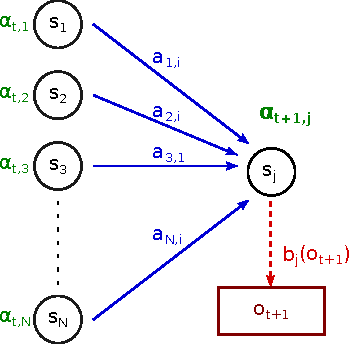
\includegraphics[width=\textwidth]{graphics/forward-backward/general/forward.pdf}
    \column{0.62\textwidth}
    \begin{itemize}
    \item Inițializare ($t = 1$)%
      \begin{equation*}
        \alpha_{1,i}=\pi_ib_i(o_1), \quad 1 \le i \le N
      \end{equation*}\pause%
    \item Inducție ($t>1$)%
      \begin{equation*}
        \label{eq:alpha_induct}
        \alpha_{t+1,j}=\Big[
        \displaystyle\sum_{i=1}^{N}\alpha_{t,j}a_{i,j}\Big]
        b_{j}(o_{t+1}), \quad \substack{1 \le t \le T-1\\1\le j \le N}
      \end{equation*}\pause%
    \item Probabilitatea secvenței observate:
      \begin{equation*}
        \label{eq:alpha_term}
        P(O \vert \lambda) =
        \displaystyle\sum_{i=1}^{N}\alpha_{T,i}
      \end{equation*}
    \end{itemize}
  \end{columns}
\end{frame}

%%%%%%%%%%%%%%%%%%%%%%
%% Slide 4: Motivația variabilelor beta
\begin{frame}
  \frametitle{Variabilele $\beta$ - Definiție}
  \begin{block}{}
    Definim variabilele $\beta$ astfel:
    \begin{equation}
      \label{eq:beta}
      \beta_{t,i}=P(o_{t+1} o_{t+2} \cdots o_{T} \vert q_t = s_i,
      \lambda)
    \end{equation}

    (probabiliatea de a fi observate valorile secvenței de la $t+1$ la
    $T$, condiționată de aflarea la momentul $t$ în starea $s_i$ și de
    parametrii $\lambda$)
  \end{block}%
  \pause%  
  \begin{block}{}
    Relația dintre $P(O \vert \lambda)$ și variabilele $\beta$ este:
    \begin{equation}
      \label{eq:eq1toalpha}
      P(O \vert \lambda) = \displaystyle\sum_{i=1}^{N}\beta_{1,i}
    \end{equation}
    (conform legii probabilităților totale)
  \end{block}%
\end{frame}

%%%%%%%%%%%%%%%%%%%%%%
%% Slide 5: Calculul variabilelor beta
\begin{frame}
  \frametitle{Calculul Variabilelor $\beta$}
  \begin{columns}[B]
    \column{0.55\textwidth}
    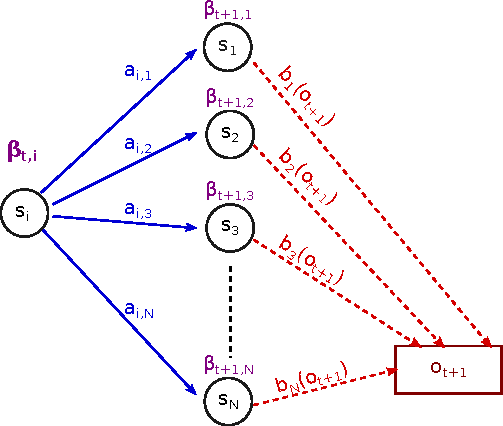
\includegraphics[width=\textwidth]{graphics/forward-backward/general/backward.pdf}
    \column{0.4\textwidth}
    \begin{itemize}
    \item Inițializare ($t=T$)
      \begin{equation}
        \beta_{T,i}=1,\quad 1 \le i \le N
        \label{eq:beta-init}
      \end{equation}
    \end{itemize}
  \end{columns}
  \begin{itemize}
  \item Pas de inducție ($t < T$) \\
    $\beta_{t,i}=\displaystyle\sum_{j=1}^{N}a_{i,j}b_j(o_{t+1})\beta_{t+1,j},
    \quad t = T-1, T-2, \ldots , 1, 1 \le i \le N$
  \end{itemize}
\end{frame}

%%%%%%%%%%%%%%%%%%%%%%
%% Slide 6: Probleme numerice
\begin{frame}
  \frametitle{Probleme numerice}
  \begin{itemize}
  \item să revedem definiția $P(O \vert \lambda)$:
    \begin{equation*}
      P(O \vert \lambda) = \displaystyle\sum_{\text{all}\;Q} \Big(
      \pi_{q_1} \cdot b_{q_1}(o_1) \cdot
      \displaystyle\prod_{t=2}^{T} b_{q_t}(o_t) a_{q_{t-1},q_t}
      \Big)
    \end{equation*}
    \pause
  \item toți cei 2$T$ factori ai unui produs sunt subunitari
  \item pentru secvențe mari, produsele se apropie mult de zero
  \item se depășește precizia disponibilă pentru reprezentare
  \item trebuie introdus un mecanism de \alert{scalare}
  \end{itemize}
\end{frame}


%%%%%%%%%%%%%%%%%%%%%%
%% Slide 7: Algoritm cu scalare
\begin{frame}
  \frametitle{Algoritmul Forward-Backward cu scalare}
  \begin{itemize}
  \item $\hat{\alpha}_{t,i}$ - variabilele $\alpha$ scalate
  \item $\hat{\beta}_{t,i}$ - variabilele $\beta$ scalate
    \vspace*{1em}
  \item $C_t$ - coeficienții de scalare \vspace*{1em}
  \item Variabilele $\alpha$ scalate
    \begin{equation}
      \label{eq:scaled-alpha}
      \hat{\alpha}_{t,i} = C_t \cdot \alpha_{t,i}
    \end{equation}
  \item Variabilele $\beta$ scalate:
    \begin{equation}
      \label{eq:scaled-beta}
      \hat{\beta}_{t,j} = C_t \cdot \beta_{t,j}
    \end{equation}
    (notațiile sunt adoptate din literatură) 
  \end{itemize}
\end{frame}

%%%%%%%%%%%%%%%%%%%%%%
%% Slide 8: Calcul alfa scalate
\begin{frame}
  \frametitle{Calculul variabilelor $\alpha$ scalate}
  \begin{columns}%
    \column{0.3\textwidth}%
    \begin{itemize}
    \item Inițializare ($t = 1$)\\\vspace*{1em}$1 \le i \le N$
    \end{itemize}%
    \column{0.7\textwidth}%
    \begin{align}%
      \ddot{\alpha}_{1,i} = \alpha_{1,i}\\
      c_1 = \frac{1}{\displaystyle\sum_{i=1}^{N}
        \ddot{\alpha}_{1,i}} \\
      \hat{\alpha}_{1,i} = c_1 \cdot \ddot{\alpha}_{1,i}
    \end{align}%
  \end{columns}%
  \vspace*{.5em} \pause \horiline
  \begin{columns}
    \column{0.3\textwidth}
    \begin{itemize}
    \item Pas de inducție ($t > 1$)\\\vspace*{1em}$1 \le i \le N$
    \end{itemize}%
    \column{0.7\textwidth}%
    \begin{align}%
      \ddot{\alpha}_{t+1,i} = \Big[
      \displaystyle\sum_{i=1}^{N}\hat{\alpha}_{t,i}a_{i,j}\Big]
      b_{j}(o_{t+1}) \\
      c_{t+1} = \dfrac{1}{\displaystyle\sum_{i=1}^{N}
        \ddot{\alpha}_{t+1,i}} \\
      \hat{\alpha}_{t+1,i} = c_{t+1} \cdot \ddot{\alpha}_{t+1,i}
    \end{align}%
  \end{columns}%
\end{frame}

%%%%%%%%%%%%%%%%%%%%%%
%% Slide 9: Coeficienți
\begin{frame}[t]
  \frametitle{Coeficienții de scalare}
  Vom nota: $C_t = c_1 \cdot c_2 \cdot \ldots \cdot c_t$\\\vspace*{1em}%
  \textbf{Ipoteza}: $\hat{\alpha}_{t,i} = C_t\alpha_{t,i}$\\\vspace*{1em}%
  \only<2-3>{%
    Demonstrație prin inducție:
    \begin{itemize}
    \item ($t=1$):
      \begin{equation*}
        \hat{\alpha}_{1,i} = c_1 \cdot \ddot{\alpha}_{1,i} = c_1 \cdot \alpha_{1,i}
      \end{equation*}%
      \visible<3>{%
      \item ($t>1$): Presupunem adevărat: $\hat{\alpha}_{t,i} = C_{t}\alpha_{t,i}$%
        \begin{align*}%
          \ddot{\alpha}_{t+1,i} & = \Big[
          \displaystyle\sum_{i=1}^{N}\hat{\alpha}_{t,i}a_{i,j}\Big]
          b_{j}(o_{t+1}) = \Big[
          \displaystyle\sum_{i=1}^{N}C_{t}\alpha_{t,i}a_{i,j}\Big]
          b_{j}(o_{t+1}) = C_{t} \alpha_{t+1,i} \\
          \hat{\alpha}_{t+1,i} & = c_{t+1} \cdot \ddot{\alpha}_{t+1,i} = c_{t+1} \cdot C_{t} \cdot\alpha_{t+1,i} = C_{t+1}\cdot\alpha_{t+1,i}
        \end{align*}%
      }%
    \end{itemize}%
  }%
  \only<4-7>{%
    Atunci:  $\mathbf{P(O \vert \lambda)} = \displaystyle\sum_{i=1}^{N}\alpha_{T,i} = 
    C^{-1}_T \cdot \displaystyle\sum_{i=1}^{N}\hat{\alpha}_{T,i} = C^{-1}_T = \mathbf{\displaystyle\prod_{t=1}^{T}c^{-1}_t}$\\\vspace*{1em}%
    \only<5-7>{%
      Calculăm $P(O \vert \lambda)$?
    }%
    \only<6-7>{%
      \textbf{\alert{NU}}\\
    }%
    \vspace*{1em}%
    \visible<7>{%
      Calculăm:
      \begin{equation}
        \label{eq:logP}
        log(P(O \vert \lambda)) = log(\displaystyle\prod_{t=1}^{T}c^{-1}_t) = \displaystyle\sum_{t=1}^{T}log(c_t^{-1}) = -\displaystyle\sum_{t=1}^{T}log(c_t)
      \end{equation}%
    }%
  }%
\end{frame}

%%%%%%%%%%%%%%%%%%%%%%
%% Slide 8: Calcul beta scalate
\begin{frame}
  \frametitle{Calculul variabilelor $\beta$ scalate}
  \begin{columns}%
    \column{0.3\textwidth}%
    \begin{itemize}
    \item Inițializare ($t = T$)\\\vspace*{1em}$1 \le i \le N$
    \end{itemize}%
    \column{0.7\textwidth}%
    \begin{align}%
      \ddot{\beta}_{T,i} = \beta_{T,i} = 1\\
      \hat{\beta}_{T,i} = c_T \cdot \ddot{\beta}_{T,i}
    \end{align}%
  \end{columns}%
  \vspace*{.5em} \pause \horiline
  \begin{columns}
    \column{0.3\textwidth}
    \begin{itemize}
    \item Pas de inducție ($t < T$)\\\vspace*{1em}$1 \le i \le N$
    \end{itemize}%
    \column{0.7\textwidth}%
    \begin{align}%
      \ddot{\beta}_{t,i} = \displaystyle\sum_{j=1}^{N}a_{i,j}b_{j}(o_{t+1})\hat{\beta}_{t+1,i}\\
      \hat{\beta}_{t,i} = c_{t} \cdot \ddot{\beta}_{t,i}
    \end{align}%
  \end{columns}%
  \begin{itemize}
  \item Se demonstrează: $\hat{\beta}_{t,i}=c_t \cdot c_{t+1} \cdot \ldots \cdot c_T \cdot \beta_{t,i}$
  \end{itemize}
\end{frame}

\begin{frame}
  \frametitle{Exemplu de aplicație}
  \begin{itemize}
    \item Să reluăm exemplul de mai devreme cu robotul.
    \item Robotul acționează diferit în fața a 2 tipuri de personalitate:
      \begin{itemize}
      \item \emph{jovialul}
      \item \emph{morocănosul}.
      \end{itemize}
    \item Pentru fiecare există un set de parametri:
      \begin{itemize}
      \item $\lambda^{1}=(A^{1},B^{1},\Pi^{1})$
      \item $\lambda^{2}=(A^{2},B^{2},\Pi^{2})$
      \end{itemize}
    \item Robotul recunoaște următoarele gesturi:\\
      \alert{(zâmbet $\vert$ rânjet)} $\longrightarrow$ \alert{(zâmbet $\vert$ rânjet)} $\longrightarrow$ \alert{încruntare}%
      \vspace*{1em}
    \item \textbf{Întrebare:} Cărei personalități este mai probabil să-i aparțină cel monitorizat?
  \end{itemize}
\end{frame}

\begin{frame}%
  \frametitle{Jovialul}%
  \begin{columns}[T]%
    \column{0.58\textwidth}%
    \only<1>{\framebox{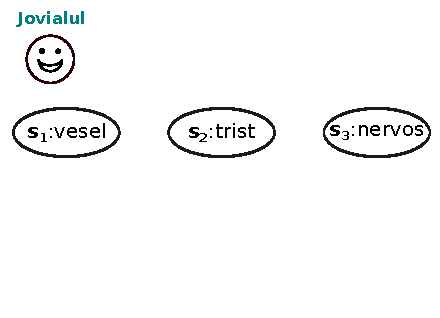
\includegraphics[width=\textwidth]{graphics/forward-backward/guys/good-guy-q.pdf}}}%
    \only<2>{\framebox{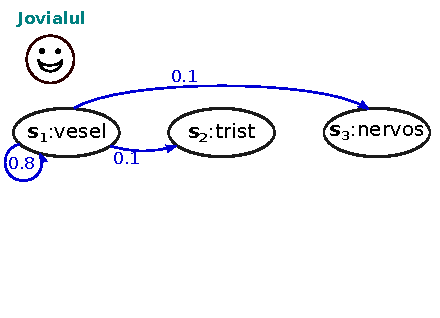
\includegraphics[width=\textwidth]{graphics/forward-backward/guys/good-guy-r.pdf}}}%
    \only<3>{\framebox{\includegraphics[width=\textwidth]{graphics/forward-backward/guys/good-guy-s.pdf}}}%
    \only<4>{\framebox{\includegraphics[width=\textwidth]{graphics/forward-backward/guys/good-guy-t.pdf}}}%
    \only<5>{\framebox{\includegraphics[width=\textwidth]{graphics/forward-backward/guys/good-guy-u.pdf}}}%
    \only<6>{\framebox{\includegraphics[width=\textwidth]{graphics/forward-backward/guys/good-guy-v.pdf}}}%
    \only<7>{\framebox{\includegraphics[width=\textwidth]{graphics/forward-backward/guys/good-guy-w.pdf}}}%
    \only<8>{\framebox{\includegraphics[width=\textwidth]{graphics/forward-backward/guys/good-guy-x.pdf}}}%
    \only<9>{\framebox{\includegraphics[width=\textwidth]{graphics/forward-backward/guys/good-guy-y.pdf}}}%
    \only<10>{\framebox{\includegraphics[width=\textwidth]{graphics/forward-backward/guys/good-guy-z.pdf}}}%
    \column{0.41\textwidth}%
    $\lambda^{1}=(A^{1},B^{1},\Pi^{1})$\\\vspace*{1em}%
    $A^{1} = \bordermatrix{~ & s_1 &
      s_2 & s_3 \cr s_1 &     \visible<2->{0.8} & \visible<2->{0.1} & \visible<2->{0.1} \cr s_2 &
      \visible<3->{0.25} & \visible<3->{0.25} & \visible<3->{0.5}
      \cr s_3 & \visible<4->{0.8} & \visible<4->{0.2} &
      \visible<4->{0} \cr}$\\\vspace*{1em}%
    $\Pi^{1} = \bordermatrix{ ~ & s_1 & s_2 & s_3 \cr ~ 
      & \visible<5->{0.7} & \visible<5->{0.2} & \visible<5->{0.1} \cr}$\\\vspace*{1em}%
    $B^{1} = \bordermatrix{~ & v_1 &
      v_2 & v_3 \cr s_1 & \visible<7->{0.7} & \visible<7->{0.3} & \visible<7->{0} \cr s_2 &
          \visible<8->{0} & \visible<8->{0.7} & \visible<8->{0.3}
          \cr s_3 & \visible<9->{0.6} & \visible<9->{0} &
          \visible<9->{0.4} \cr}$
  \end{columns}%
\end{frame}%

\begin{frame}%
  \frametitle{Morocănosul}%
  \begin{columns}[T]%
    \column{0.58\textwidth}%
    \only<1>{\framebox{\includegraphics[width=\textwidth]{graphics/forward-backward/guys/surly-guy-q.pdf}}}%
    \only<2>{\framebox{\includegraphics[width=\textwidth]{graphics/forward-backward/guys/surly-guy-r.pdf}}}%
    \only<3>{\framebox{\includegraphics[width=\textwidth]{graphics/forward-backward/guys/surly-guy-s.pdf}}}%
    \only<4>{\framebox{\includegraphics[width=\textwidth]{graphics/forward-backward/guys/surly-guy-t.pdf}}}%
    \only<5>{\framebox{\includegraphics[width=\textwidth]{graphics/forward-backward/guys/surly-guy-u.pdf}}}%
    \only<6>{\framebox{\includegraphics[width=\textwidth]{graphics/forward-backward/guys/surly-guy-v.pdf}}}%
    \only<7>{\framebox{\includegraphics[width=\textwidth]{graphics/forward-backward/guys/surly-guy-w.pdf}}}%
    \only<8>{\framebox{\includegraphics[width=\textwidth]{graphics/forward-backward/guys/surly-guy-x.pdf}}}%
    \only<9>{\framebox{\includegraphics[width=\textwidth]{graphics/forward-backward/guys/surly-guy-y.pdf}}}%
    \only<10>{\framebox{\includegraphics[width=\textwidth]{graphics/forward-backward/guys/surly-guy-z.pdf}}}%
    \column{0.41\textwidth}%
    $\lambda^{2}=(A^{2},B^{2},\Pi^{2})$\\\vspace*{1em}%
    $A^{2} = \bordermatrix{~ & s_1 &
      s_2 & s_3 \cr s_1 &     \visible<2->{0.5} & \visible<2->{0.3} & \visible<2->{0.2} \cr s_2 &
      \visible<3->{0.1} & \visible<3->{0.6} & \visible<3->{0.3}
      \cr s_3 & \visible<4->{0.4} & \visible<4->{0.5} &
      \visible<4->{0.1} \cr}$\\\vspace*{1em}%
    $\Pi^{2} = \bordermatrix{ ~ & s_1 & s_2 & s_3 \cr ~ 
      & \visible<5->{0.3} & \visible<5->{0.5} & \visible<5->{0.2} \cr}$\\\vspace*{1em}%
    $B^{2} = \bordermatrix{~ & v_1 &
      v_2 & v_3 \cr s_1 & \visible<7->{0.4} & \visible<7->{0.5} & \visible<7->{0.1} \cr s_2 &
          \visible<8->{0} & \visible<8->{0.2} & \visible<8->{0.8}
          \cr s_3 & \visible<9->{0.6} & \visible<9->{0} &
          \visible<9->{0.4} \cr}$
  \end{columns}%
\end{frame}%

\begin{frame}
  \frametitle{Calculul variabilelor $\alpha$:}%
  \begin{columns}%
    \column{0.57\textwidth}
    \only<1>{\framebox{\includegraphics[width=\textwidth]{graphics/forward-backward/compute-alpha/compute-alpha-none.pdf}}}%
    \only<2>{\framebox{\includegraphics[width=\textwidth]{graphics/forward-backward/compute-alpha/compute-alpha-11.pdf}}}%
    \only<3>{\framebox{\includegraphics[width=\textwidth]{graphics/forward-backward/compute-alpha/compute-alpha-12.pdf}}}%
    \only<4>{\framebox{\includegraphics[width=\textwidth]{graphics/forward-backward/compute-alpha/compute-alpha-13.pdf}}}%
    \only<5-6>{\framebox{\includegraphics[width=\textwidth]{graphics/forward-backward/compute-alpha/compute-alpha-1.pdf}}}%
    \only<7>{\framebox{\includegraphics[width=\textwidth]{graphics/forward-backward/compute-alpha/compute-alpha-21.pdf}}}%
    \only<8>{\framebox{\includegraphics[width=\textwidth]{graphics/forward-backward/compute-alpha/compute-alpha-22.pdf}}}%
    \only<9>{\framebox{\includegraphics[width=\textwidth]{graphics/forward-backward/compute-alpha/compute-alpha-23.pdf}}}%
    \only<10-11>{\framebox{\includegraphics[width=\textwidth]{graphics/forward-backward/compute-alpha/compute-alpha-2.pdf}}}%
    \only<12>{\framebox{\includegraphics[width=\textwidth]{graphics/forward-backward/compute-alpha/compute-alpha-31.pdf}}}%
    \only<13>{\framebox{\includegraphics[width=\textwidth]{graphics/forward-backward/compute-alpha/compute-alpha-32.pdf}}}%
    \only<14>{\framebox{\includegraphics[width=\textwidth]{graphics/forward-backward/compute-alpha/compute-alpha-33.pdf}}}%
    \only<15-16>{\framebox{\includegraphics[width=\textwidth]{graphics/forward-backward/compute-alpha/compute-alpha-3.pdf}}}%
    \vspace*{2em}%
     \\$\hat{\alpha} = \begin{bmatrix}
       \scriptstyle \visible<6->{0.8909} & \scriptstyle \visible<6->{0} & \scriptstyle \visible<6->{0.1091} \\
       \scriptstyle \visible<11->{0.9128} & \scriptstyle \visible<11->{0} & \scriptstyle \visible<11->{0.0872} \\
       \scriptstyle \visible<16->{0} & \scriptstyle \visible<16->{0.4718} & \scriptstyle \visible<16->{0.5282}\end{bmatrix} \:
     c = \begin{bmatrix} 
      \scriptstyle \visible<5->{1.8182} \\ 
      \scriptstyle \visible<10->{1.63} \\ 
      \scriptstyle \visible<15->{14.4718}\end{bmatrix}$
    \vspace*{3em}%
    \column{0.43\textwidth}
    \only<2-6>{%
      \begin{align*}
        \scriptstyle \ddot{\alpha}_{1,1}=\pi_{1,1}\cdot b_1(v_1)=0.7\cdot 0.7 = 0.49 \\
        \visible<3->{%
          \scriptstyle \ddot{\alpha}_{1,2}=\pi_{1,2}\cdot b_2(v_1)=0.2\cdot 0 = 0 \\
        }
        \visible<4->{%
          \scriptstyle \ddot{\alpha}_{1,3}=\pi_{1,3}\cdot b_3(v_1)=0.1\cdot 0.6 = 0.6 \\
        }%
      \end{align*}%
      \visible<5->{%
        \vspace*{-4em}\horiline\vspace*{-.5em}%
        \begin{align*}
          \scriptstyle c_1 & \scriptstyle = \frac{1}{\ddot{\alpha}_{1,1} + \ddot{\alpha}_{1,2} +
            \ddot{\alpha}_{1,3}} \\\scriptstyle c_1 & \scriptstyle  = 1 / 0.54 \approx 1.8182
        \end{align*}%
        \visible<6->{%
          \vspace*{-2.5em}\horiline\vspace*{-.5em}%
          \begin{align*}
            \scriptstyle \hat{\alpha}_{1,1} & \scriptstyle = c_1 \cdot \ddot{\alpha}_{1,1} = 0.8909 \\
            \scriptstyle \hat{\alpha}_{1,2} & \scriptstyle = c_1 \cdot \ddot{\alpha}_{1,2} = 0\\
            \scriptstyle \hat{\alpha}_{1,3} & \scriptstyle = c_1 \cdot \ddot{\alpha}_{1,3} = 0.1091
          \end{align*}%
        }%
      }%
    }%
    \only<7-11>{%
      \begin{align*}%
        \scriptstyle \ddot{\alpha}_{2,1} & \scriptstyle =b_1(v_1)\sum\hat{\alpha}_{1,i}a_{i,1} \\
        & \scriptstyle = \ldots = 0.56 \\
        \visible<8->{%
          \scriptstyle \ddot{\alpha}_{2,2} & \scriptstyle =b_2(v_1) \sum \hat{\alpha}_{1,i}a_{i,2} = 0\\
        }%
        \visible<9->{%
          \scriptstyle \ddot{\alpha}_{2,3} & \scriptstyle =b_3(v_1) \sum \hat{\alpha}_{1,i}a_{i,3} = 0.0535
        }%
      \end{align*}%
      \visible<10->{%
        \vspace*{-2.5em}\horiline\vspace*{-.5em}%
        \begin{align*}
          \scriptstyle c_2 & \scriptstyle = \frac{1}{\ddot{\alpha}_{2,1} + \ddot{\alpha}_{2,2} + \ddot{\alpha}_{2,3}} \\\scriptstyle c_2 & \scriptstyle  = \frac{1}{0.484+0.0776+0} = 1.63
        \end{align*}%
        \visible<11->{%
          \vspace*{-2.5em}\horiline\vspace*{-.5em}%
          \begin{align*}
            \scriptstyle \hat{\alpha}_{2,1} & \scriptstyle = c_2 \cdot \ddot{\alpha}_{2,1} = 0.9128 \\
            \scriptstyle \hat{\alpha}_{2,2} & \scriptstyle =c_2 \cdot \ddot{\alpha}_{2,2} = 0 \\
            \scriptstyle \hat{\alpha}_{2,3} & \scriptstyle =c_2 \cdot \ddot{\alpha}_{2,3} = 0.0872
          \end{align*}%
        }%
      }%
    }%
    \only<12-16>{%
      \begin{align*}%
        \scriptstyle \ddot{\alpha}_{3,1} & \scriptstyle =b_1(v_3)\sum\hat{\alpha}_{2,i}a_{i,1} \\
        & \scriptstyle = \ldots = 0 \\
        \visible<13->{%
          \scriptstyle \ddot{\alpha}_{3,2} & \scriptstyle =b_2(v_3) \sum \hat{\alpha}_{2,i}a_{i,2} = 0.0326\\
        }%
        \visible<14->{%
          \scriptstyle \ddot{\alpha}_{3,3} & \scriptstyle =b_3(v_3) \sum \hat{\alpha}_{2,i}a_{i,3} = 0.0365
        }%
      \end{align*}%
      \visible<15->{%
        \vspace*{-2.5em}\horiline\vspace*{-.5em}%
        \begin{align*}
          \scriptstyle c_3 & \scriptstyle = \frac{1}{\ddot{\alpha}_{3,1} + \ddot{\alpha}_{3,2} + \ddot{\alpha}_{,3}} \\\scriptstyle c_3 & \scriptstyle  = \frac{1}{0.069} = 14.4718
        \end{align*}%
        \visible<16->{%
          \vspace*{-2.5em}\horiline\vspace*{-.5em}%
          \begin{align*}
            \scriptstyle \hat{\alpha}_{3,1} & \scriptstyle = c_3 \cdot \ddot{\alpha}_{3,1} = 0 \\
            \scriptstyle \hat{\alpha}_{3,2} & \scriptstyle =c_3 \cdot \ddot{\alpha}_{3,2} = 0.4718 \\
            \scriptstyle \hat{\alpha}_{3,3} & \scriptstyle =c_3 \cdot \ddot{\alpha}_{3,3} = 0.5282
          \end{align*}%
        }%
      }%
    }%
  \end{columns}%
\end{frame}

\begin{frame}
  \frametitle{Morocănos sau jovial?}
  \begin{itemize}
    \item $c = \begin{bmatrix} \scriptstyle 1.8182 & \scriptstyle 1.63 &  \scriptstyle 14.4718\end{bmatrix}$
    \item Probabilitatea ca secvența observată să fi fost generată de un \emph{jovial}:\\
      $\log(P(O\vert \lambda^{1}))=-\displaystyle\sum\log(c_i) = -3.7583$\\\vspace*{1em}\pause%
    \item Probabilitatea ca secvența observată să fi fost generată de un \emph{morocănos}:\\
      $\log(P(O\vert \lambda^{2}))=-3.6362$\\\vspace*{1em}%\pause
    \item $\log(P(O\vert \lambda^{2})) > \log(P(O\vert \lambda^{1}))$
    \item Este mai probabil să avem de-a face cu un...\pause\\\vspace*{.5em}%
      \begin{center}\includegraphics{graphics/forward-backward/guys/surly-face.pdf}\end{center}
    \end{itemize}
\end{frame}

\begin{frame}
  \frametitle{Calculul variabilelor $\beta$:}
    \begin{columns}%
    \column{0.6\textwidth}
    \only<1>{\framebox{\includegraphics[width=\textwidth]{graphics/forward-backward/compute-beta/compute-beta-none.pdf}}}%
    \only<2>{\framebox{\includegraphics[width=\textwidth]{graphics/forward-backward/compute-beta/compute-beta-31.pdf}}}%
    \only<3>{\framebox{\includegraphics[width=\textwidth]{graphics/forward-backward/compute-beta/compute-beta-32.pdf}}}%
    \only<4>{\framebox{\includegraphics[width=\textwidth]{graphics/forward-backward/compute-beta/compute-beta-33.pdf}}}%
    \only<5>{\framebox{\includegraphics[width=\textwidth]{graphics/forward-backward/compute-beta/compute-beta-21.pdf}}}%
    \only<6>{\framebox{\includegraphics[width=\textwidth]{graphics/forward-backward/compute-beta/compute-beta-22.pdf}}}%
    \only<7>{\framebox{\includegraphics[width=\textwidth]{graphics/forward-backward/compute-beta/compute-beta-23.pdf}}}%
    \only<8>{\framebox{\includegraphics[width=\textwidth]{graphics/forward-backward/compute-beta/compute-beta-11.pdf}}}%
    \only<9>{\framebox{\includegraphics[width=\textwidth]{graphics/forward-backward/compute-beta/compute-beta-12.pdf}}}%
    \only<10>{\framebox{\includegraphics[width=\textwidth]{graphics/forward-backward/compute-beta/compute-beta-13.pdf}}}%
  \end{columns}%
\end{frame}


\begin{frame}[fragile]
  \frametitle{Algoritmul Forward-Backward} \vspace*{-1em}
  \begin{columns}[T]
    \column{0.5\textwidth}
    \begin{algorithm}[H]
      \scriptsize
      \caption{Calculul variabilelor $\alpha$}
      \label{alg1}
      \algsetup{linenosize=\tiny} \algsetup{indent=2.25em}
      \begin{algorithmic}[2]
        \FOR{$i=1$ to $N$} \STATE $\ddot{\alpha}_{1,i} \leftarrow
        \pi_i \cdot b_i(o_1)$
        \ENDFOR
        \STATE $c_1 \leftarrow (\displaystyle\sum_{i=1}^{N}
        \ddot{\alpha}_{1,i})^{-1}$ \FOR{$i=1$ to $N$} \STATE
        $\hat{\alpha}_{1,i} \leftarrow c_1 \cdot \ddot{\alpha}_{1,i}$
        \ENDFOR
        \FOR{$t=1$ to $T-1$} \FOR{$i=1$ to $N$} \STATE
        $\ddot{\alpha}_{t+1,i} \leftarrow \Big[
        \displaystyle\sum_{i=1}^{N}\hat{\alpha}_{t,i}a_{i,j}\Big]
        b_{j}(o_{t+1})$
        \ENDFOR
        \STATE $c_{t+1} \leftarrow (\displaystyle\sum_{i=1}^{N}
        \ddot{\alpha}_{t+1,i})^{-1}$ \FOR{$i=1$ to $N$} \STATE
        $\hat{\alpha}_{t+1,i} \leftarrow c_{t+1} \cdot
        \ddot{\alpha}_{t+1,i}$
        \ENDFOR
        \ENDFOR
      \end{algorithmic}
    \end{algorithm}
    \column{0.5\textwidth}
    \begin{algorithm}[H]
      \scriptsize
      \caption{Calculul $P(O \vert \lambda)$}
      \label{alg2}
      \algsetup{linenosize=\tiny} \algsetup{indent=2em}
      \begin{algorithmic}[2]
        \STATE $logP \leftarrow -\displaystyle\sum_{t=1}^{T}c_t$
      \end{algorithmic}
    \end{algorithm}
    \vspace*{1em}
    \begin{algorithm}[H]
      \scriptsize
      \caption{Calculul variabilelor $\beta$}
      \label{alg3}
      \algsetup{linenosize=\tiny} \algsetup{indent=2em}
      \algsetup{linenosize=\tiny}
      \begin{algorithmic}[2]
        \FOR{$i=1$ to $N$} \STATE $\hat{\beta}_{T,i} \leftarrow \cdot
        c_T$
        \ENDFOR
        \FOR{$t=(T-1)$ to $1$} \FOR{$i=1$ to $N$} \STATE
        $\hat{\beta}_{t,i} \leftarrow \displaystyle\sum_{j=1}^{N}
        a_{i,j} b_{j}(o_{t+1}) \hat{\beta}_{t+1,j} \cdot c_t$
        \ENDFOR
        \ENDFOR
      \end{algorithmic}
    \end{algorithm}
  \end{columns}
\end{frame}

\begin{frame}
  \frametitle{A venit vremea să scriem cod}
  \begin{enumerate}
  \item Faceți o copie a fișierului \texttt{forward\_backward\_disc.m.stub} 
    și denumiți-o \texttt{forward\_backward\_disc.m} (eliminați sufixul \texttt{.stub}).
    \\Veți implementa funcția:\\
    \mcode{function [logP, Alpha, Beta, Scale] = forward_backward_disc(O,Pi, A, B)}
    \pause
  \item Completați cele trei secțiuni (calcul $Alpha$, $Beta$ și $logP$).%
    \vspace*{-.5em}
    \lstinputlisting{m-files/forward.m}
\item Folosiți \mcode{hmm_test} pentru a vă testa codul.
\end{enumerate}
\end{frame}


\subsection{Problema Interpretării: Algoritmul Viterbi}
\label{sec:viterbi}

%% tudor
%% Tudor Berariu, Alexandru Sorici
%% Noiembrie 2012


\begin{frame}
  \frametitle{Problema interpretării}
  \begin{block}{Problema interpretării unei secvențe de observații}
    Date fiind un model   \alert{$\lambda=(A,B,\Pi)$} și o
    secvență de observații \alert{$O = [ o_1 o_2 \cdots o_T ]$}, 
    cum alegem o secvență corespunzătoare de stări
    \alert{$Q_{\text{best}} = [ q_{1_{\text{best}}} q_{2_{\text{best}}} \cdots q_{T_{\text{best}}} ]$} care \emph{să
      dea un înțeles} observațiilor? Cum \emph{descoperim} partea
    ascunsă a modelului?
  \end{block}\pause
  \begin{itemize}
  \item Răspunsul depinde de criteriul cu care alegem \emph{cea mai bună} secvență\pause
    \begin{itemize}
    \item \alert{secvența celor mai probabile stări $q_{t_{\text{best}}}$} (luate individual), date fiind modelul și secvența observată:\\
      $q_{t_{\text{best}}} = \underset{s_i}{\operatorname{argmax}}\; P(q_t = s_i \vert O, \lambda)$
    \item \alert{cea mai probabilă secvență de stări $Q$} (per ansamblu), date fiind modelul și secvența observată:\\
      $Q_{\text{best}} = \underset{\text{all }Q}{\operatorname{argmax}}\; P(Q \vert O, \lambda)$
    \end{itemize}
  \end{itemize}
\end{frame}


\begin{frame}
  \frametitle{Secvența celor mai probabile stări}
  Notație: $P(q_t = s_i \vert O, \lambda) = \mathbf{\gamma_{t,i}} = 
  \frac{\alpha_{t,i}\beta_{t,i}}{\displaystyle\sum_{j=1}^{N}\alpha_{t,j}\beta_{t,j}}$
  \begin{itemize}
  \item Este un criteriu satisfăcător?\pause
  \item \textbf{NU!}\\Pot exista $q_t$ și $q_{t+1}$ astfel încât $a_{q_t,q_{t+1}}=0$
  \end{itemize}
    % \begin{itemize}      
  % \item How can we answer the \emph{best explanation} problem?  \pause
  % \item \textbf{Individually} most likely states
  %   \begin{equation}
  %     \label{eq:individually}
  %     \gamma_{t,i}=P(q_t = s_i \vert O, \lambda)
  %   \end{equation}
  %   \pause
  % \item Computation
  %   \begin{equation}
  %     \label{eq:gamma_formula}
  %     \gamma_{t,i}=\frac{\alpha_{t,i}\beta_{t,i}}{P(O\vert \lambda)} =
  %     \frac{\alpha_{t,i}\beta_{t,i}}{\displaystyle\sum_{k=1}^{N}\alpha_{t,k}\beta_{t,k}}
  %   \end{equation}
  %   \pause
  % \item Problems?
  % \end{itemize}

\end{frame}

\begin{frame}
  \frametitle{Algoritmul Viterbi}
  \begin{itemize}
  \item Criteriu care ia în considerare distribuțiile de probabilitate 
    ale tranzițiilor între stări
  \item Cea mai bună cale:
    $Q_{\text{best}} = [q_{1_{\text{best}}} q_{2_{\text{best}}} \cdots q_{T_{\text{best}}}]$
    \begin{equation}
      Q_{\text{best}} = \underset{Q}{\operatorname{argmax}}\;
      P(Q \vert O, \lambda)
      = \underset{Q}{\operatorname{argmax}}\; P(Q, O \vert \lambda)
      \tag{\ref{eq:best-explanation}}
    \end{equation}
  \item \textbf{Algoritmul Viterbi} - programare dinamică
  \item Vom introduce variabilele $delta$.
  \end{itemize}
\end{frame}

\begin{frame}
  \frametitle{Variabilele $\delta$ - intuiție}
  \begin{block}{Întrebare}
    Dacă $Q = [q_1, q_2, \ldots, q_{t-1}, q_{t}]$ este cea mai bună secvență care explică $O = [o_1, o_2, \ldots o_{t-1}, o_{t}]$, atunci putem afirma că $Q[1:t-1]$ este cea mai bună secvență de stări care explică $O[1:t-1]$?
  \end{block}
  \pause
  \vspace*{1em}
  \begin{itemize}
  \item \textbf{NU!}
    \begin{align*}
        & P(q_1 = s_{i_1}, q_2 = s_{i_2}, \ldots, q_{t-1} = s_{i_{t-1}}, q_{t} = s_{i_{t}}\vert O, \lambda) = \\
        & P(q_1, q_2, \ldots, q_{t-1} \vert O, \lambda) \cdot  P(q_t = s_{i_t} \vert q_{t-1}= s_{i_{t-1}}, \lambda) \cdot P(o_t \vert q_t=s_{i_t}, \lambda)
      \end{align*}
    \end{itemize}
\end{frame}

\begin{frame}
  \frametitle{Variabilele $\delta$}
  \begin{itemize}
  \item Vom numi variabile $\delta$:
    \begin{equation}
      \label{eq:delta-definition}
      \delta_{t,i}=\underset{q_1,\ldots,q_{t-1}}{\operatorname{max}}
      P([q_1 q_2 \ldots q_{t-1} s_i], [o_1, o_2, \ldots o_t] \vert \lambda)
    \end{equation}
  \end{itemize}
  \begin{columns}
    \column{0.45\textwidth}
    \begin{itemize}
    \item $\mathbf{\delta_{t,i}}$ - cea mai mare probabilitate a unei secvențe de 
      stări de lungime $t$ care ajunge în $s_i$ și explică primele $t$ valori observate
      \visible<2>{
      \item relația dintre variabilele $\delta$:
        \begin{equation}
          \label{eq:delta-recurrence}
          \delta_{t+1,j} = [\underset{i}{\operatorname{max}}\; 
          \delta_{t,i} \cdot a_{i,j}] \cdot b_{j}(o_{t+1})
        \end{equation}}
    \end{itemize}
    \column{0.45\textwidth} \visible<2>{
      \includegraphics[width=\textwidth]{graphics/viterbi/general/viterbi-path.pdf}
    }
  \end{columns}
\end{frame}

\begin{frame}
  \frametitle{Algoritmul Viterbi - Privire de ansamblu}
  \begin{block}{Pași înainte}
    Calculăm cea mai mare probabilitate de a ajunge în starea $s_i$ 
    la momentul $t$ pe baza celor mai mari probabilități de a fi ajuns în 
    toate stările $s_j$ la $t-1$.
  \end{block}
  \pause
  \begin{block}{La final ($t=T$)}
    Starea finală este acea stare $s_i$ cu cea mai mare probabilitate de a ajunge
    la ea după observarea tuturor valorilor.
  \end{block}
  \pause
  \begin{block}{Pași înapoi}
    Refacem \emph{cea mai bună cale} alegând pentru fiecare moment $t$ starea care a
    dus la probabilitatea maximă pentru starea de la $t+1$.
  \end{block}
\end{frame}

\begin{frame}
  \frametitle{Algoritmul Viterbi (I)}
  \begin{description}
  \item[1] Inițializare: \\
    \begin{equation}
      \label{eq:viterbi-initialization}
      \begin{split}
        \delta_{1,i} & = \pi_{i}b_i(o_1), \quad 1 \le i \le N \\
        \psi_{1,i} & = 0
      \end{split}
    \end{equation}
  \item[2] Recursivitate: \\
    \begin{equation}
      \label{eq:viterbi-recursion}
      \begin{split}
        \delta_{t,j} & = [\underset{i }{\operatorname{max}}\; \delta_{t-1,i} \cdot
        a_{i,j}] \cdot b_{j}(o_{t})
        \quad \scriptstyle{2 \le t \le T, 1 \le j \le N} \\
        \psi_{t,i} & = \underset{i}{\operatorname{argmax}}\; \delta_{t-1,i}\cdot
        a_{i,j} \quad \scriptstyle{2 \le t \le T, 1 \le j \le N}
      \end{split}
    \end{equation}
  \end{description}
\end{frame}

\begin{frame}
  \frametitle{Algoritmul Viterbi (II)}
  \begin{description}
  \item[3] Terminare: \\
    \begin{equation}
      \label{eq:viterbi-termination}
      \begin{split}
        P(Q_{\text{best}} \vert O, \lambda) & = \underset{i}{\operatorname{max}}\; \delta_{T,i} \\
        q_{T_{\text{best}}} & = \underset{i}{\operatorname{argmax}}\; \delta_{T,i}
      \end{split}
    \end{equation}
  \item[4] Backtracking: \\
    \begin{equation}
      \label{eq:viterbi-backtracking}
      q_{t_{\text{best}}} = \psi_{t+1}(q_{t+1_{\text{best}}}), \quad \scriptstyle{t=T-1,T-2,\cdots, 1}
    \end{equation}
  \end{description}
\end{frame}

\begin{frame}
  \frametitle{Probleme numerice}
  \begin{itemize}
  \item Cine este $P(Q_{\text{best}} \vert O, \lambda)$?
    \begin{equation*}
      \begin{split}
        P(Q_{\text{best}} \vert O, \lambda) & = \delta_{T,i_T} \\
        P(Q_{\text{best}} \vert O, \lambda) & = \delta_{T-1,i_{T-1}} \cdot a_{i_{T-1},i_T} 
        \cdot b_{T}(o_{T})\\
        P(Q_{\text{best}} \vert O, \lambda) & = \delta_{T-2,i_{T-2}} \cdot a_{i_{T-2},i_{T-1}}
        \cdot b_{T-1}(o_{T-1}) \cdot a_{i_{T-1},j_T} \cdot b_{T}(o_{T})\\
        P(Q_{\text{best}} \vert O, \lambda) & = \displaystyle\prod \ldots
      \end{split}
    \end{equation*}
  \item Cum putem evita apropierea rapidă de zero?\pause
  \item Calculăm \alert{$log(P)$}
    \begin{equation*}
      \begin{split}
        \log(P(Q_{\text{best}} \vert O, \lambda)) & = \log(\delta_{T,i_T}) \\
        \log(P(Q_{\text{best}} \vert O, \lambda)) & = \log(\delta_{T-1,i_{T-1}}) + \log(a_{i_{T-1},i_T})
        + \log(b_{T}(o_{T}))\\
        \log(P(Q_{\text{best}} \vert O, \lambda)) & = \log(\delta_{T-2,i_{T-2}}) + \log(a_{i_{T-2},i_{T-1}})
        +\log(b_{T-1}(o_{T-1})+\log(a_{i_{T-1},j_T})+\log(b_{T}(o_{T}))\\
        \log(P(Q_{\text{best}} \vert O, \lambda)) & = \displaystyle\sum \ldots
      \end{split}
    \end{equation*}
    
  \end{itemize}
\end{frame}

\begin{frame}
  \frametitle{Probleme numerice - Rezolvare}
  \begin{itemize}
  \item Notație:
    \begin{equation*}
      \phi_{t,i}=\underset{q_1,\ldots,q_{t-1}}{\operatorname{max}}
      \log(P(q_1,\ldots,q_{t-1},q_t=s_i,o_1,\ldots,o_t\vert \lambda))=\log(\delta_{t,i})
    \end{equation*}
  \item Matricele $\log(\Pi)$, $\log(A)$ și $\log(B)$ pot fi precalculate.
  \end{itemize}
\end{frame}

\begin{frame}
  \frametitle{Algoritmul Viterbi - $log(P)$ (I)}
  \begin{description}
  \item[1] Inițializare: \\
    \begin{equation}
      \label{eq:viterbi-initialization}
      \begin{split}
        \phi_{1,i} & = \log(\pi_{i}) \mathbf{+} \log(b_i(o_1)), \quad 1 \le i \le N \\
        \psi_{1,i} & = 0
      \end{split}
    \end{equation}
  \item[2] Recursivitate: \\
    \begin{equation}
      \label{eq:viterbi-recursion}
      \begin{split}
        \phi_{t,j} & = [\underset{i}{\operatorname{max}}\; \phi_{t-1,i} \mathbf{+}
        log(a_{i,j})] \mathbf{+} \log(b_{j}(o_{t}))
        \quad \scriptstyle{2 \le t \le T, 1 \le j \le N} \\
        \psi_{t,i} & = \underset{i}{\operatorname{argmax}}\; \phi_{t-1,i} \mathbf{+}
        \log(a_{i,j}) \quad \scriptstyle{2 \le t \le T, 1 \le j \le N}
      \end{split}
    \end{equation}
  \end{description}
\end{frame}

\begin{frame}
  \frametitle{Algoritmul Viterbi - $log(P)$ (II)}
  \begin{description}
  \item[3] Terminare: \\
    \begin{equation}
      \label{eq:viterbi-termination}
      \begin{split}
        \log(P(Q_{\text{best}} \vert O, \lambda)) & = \underset{i}{\operatorname{max}}\; \phi_{T,i} \\
        q_{T_{\text{best}}} & = \underset{i}{\operatorname{argmax}}\; \phi_{T,i}
      \end{split}
    \end{equation}
  \item[4] Backtracking: \\
    \begin{equation}
      \label{eq:viterbi-backtracking}
      q_{t_{\text{best}}} = \psi_{t+1}(q_{t+1_{\text{best}}}), \quad \scriptstyle{t=T-1,T-2,\cdots, 1}
    \end{equation}
  \end{description}
\end{frame}

\begin{frame}
  \frametitle{Înapoi la exemplu}
  \begin{itemize}
  \item Să reluăm exemplul cu robotul.
  \item Robotul a recunoscut secvența de gesturi:\\
      \alert{(zâmbet $\vert$ rânjet)} $\longrightarrow$ \alert{(zâmbet $\vert$ rânjet)} $\longrightarrow$ \alert{încruntare}
  \item Am stabilit:
    $P(O \vert \lambda^{1}) > P(O \vert \lambda^{2})$\pause\\
    Deci, robotul se confruntă \emph{[, probabil]} cu un morocănos!\\
  \item A doua întrebare: \textbf{Prin ce stări a trecut acesta?}
  \end{itemize}
\end{frame}

\begin{frame}%
  \frametitle{Jovialul}%
  \begin{columns}[T]%
    \column{0.70\textwidth}%
    \only<1>{\framebox{\includegraphics[width=\textwidth]{graphics/viterbi/compute-viterbi/compute-viterbi-none.pdf}}}%
    \only<2>{\framebox{\includegraphics[width=\textwidth]{graphics/viterbi/compute-viterbi/compute-viterbi-11.pdf}}}%
    \only<3>{\framebox{\includegraphics[width=\textwidth]{graphics/viterbi/compute-viterbi/compute-viterbi-12.pdf}}}%
    \only<4>{\framebox{\includegraphics[width=\textwidth]{graphics/viterbi/compute-viterbi/compute-viterbi-13.pdf}}}%
    \only<5>{\framebox{\includegraphics[width=\textwidth]{graphics/viterbi/compute-viterbi/compute-viterbi-21a.pdf}}}%
    \only<6>{\framebox{\includegraphics[width=\textwidth]{graphics/viterbi/compute-viterbi/compute-viterbi-21b.pdf}}}%
    \only<7>{\framebox{\includegraphics[width=\textwidth]{graphics/viterbi/compute-viterbi/compute-viterbi-22a.pdf}}}%
    \only<8>{\framebox{\includegraphics[width=\textwidth]{graphics/viterbi/compute-viterbi/compute-viterbi-22b.pdf}}}%
    \only<9>{\framebox{\includegraphics[width=\textwidth]{graphics/viterbi/compute-viterbi/compute-viterbi-23a.pdf}}}%
    \only<10>{\framebox{\includegraphics[width=\textwidth]{graphics/viterbi/compute-viterbi/compute-viterbi-23b.pdf}}}%
    \only<11>{\framebox{\includegraphics[width=\textwidth]{graphics/viterbi/compute-viterbi/compute-viterbi-31a.pdf}}}%
    \only<12>{\framebox{\includegraphics[width=\textwidth]{graphics/viterbi/compute-viterbi/compute-viterbi-31b.pdf}}}%
    \only<13>{\framebox{\includegraphics[width=\textwidth]{graphics/viterbi/compute-viterbi/compute-viterbi-32a.pdf}}}%
    \only<14>{\framebox{\includegraphics[width=\textwidth]{graphics/viterbi/compute-viterbi/compute-viterbi-32b.pdf}}}%
    \only<15>{\framebox{\includegraphics[width=\textwidth]{graphics/viterbi/compute-viterbi/compute-viterbi-33a.pdf}}}%
    \only<16>{\framebox{\includegraphics[width=\textwidth]{graphics/viterbi/compute-viterbi/compute-viterbi-33b.pdf}}}%
    \only<17>{\framebox{\includegraphics[width=\textwidth]{graphics/viterbi/compute-viterbi/compute-viterbi-3.pdf}}}%
    \only<18>{\framebox{\includegraphics[width=\textwidth]{graphics/viterbi/compute-viterbi/compute-viterbi-2.pdf}}}%
    \only<19>{\framebox{\includegraphics[width=\textwidth]{graphics/viterbi/compute-viterbi/compute-viterbi-1.pdf}}}%
    \column{0.30\textwidth}%
    \only<2>{%
      \begin{equation*}
        \begin{split}
          \scriptstyle \phi_{1,1} & \scriptstyle  = \log(\pi_{1}) + \log(b_{1,1})
      \end{split}
    \end{equation*}
    \vspace*{2em}
    \begin{equation*}
      \begin{split}
        \scriptstyle \psi_{1,1} & \scriptstyle  = 0
      \end{split}
    \end{equation*}
    }\only<3>{%
      \begin{equation*}
      \begin{split}
        \scriptstyle \phi_{1,2} & \scriptstyle  = \log(\pi_{2}) + \log(b_{2,1})
      \end{split}
    \end{equation*}
    \vspace*{2em}
    \begin{equation*}
      \begin{split}
        \scriptstyle \psi_{1,2} & \scriptstyle  = 0
      \end{split}
    \end{equation*}
    }\only<4>{%
      \begin{equation*}
      \begin{split}
        \scriptstyle \phi_{1,3} & \scriptstyle  = \log(\pi_{3}) + \log(b_{3,1})
      \end{split}
    \end{equation*}
    \vspace*{2em}
    \begin{equation*}
      \begin{split}
        \scriptstyle \psi_{1,3} & \scriptstyle  = 0
      \end{split}
    \end{equation*}
    }\only<5>{%
      \begin{equation*}
      \begin{split}
        \scriptstyle \phi_{1,3} & \scriptstyle  = \operatorname{max} \Big\lbrace \\
        \scriptstyle & \scriptstyle \log(\phi_{1,1}) + \log(a_{1,1}),\\ 
        \scriptstyle & \scriptstyle \log(\phi_{2,1}) + \log(a_{2,1}),\\
        \scriptstyle & \scriptstyle \log(\phi_{1,3}) + \log(a_{3,1}) \Big\rbrace \\ 
        \scriptstyle & \scriptstyle + \log(b_{1,1})
      \end{split}
    \end{equation*}
    % \begin{equation*}
    %   \begin{split}
    %     \scriptstyle \psi_{1,3} & \scriptstyle  = \operatorname{argmax} \Big\lbrace \\
    %     \scriptstyle & \scriptstyle \log(\phi_{1,1}) + \log(a_{1,1}),\\ 
    %     \scriptstyle & \scriptstyle \log(\phi_{2,1}) + \log(a_{2,1}),\\
    %     \scriptstyle & \scriptstyle \log(\phi_{1,3}) + \log(a_{3,1}) \Big\rbrace \\
    %   \end{split}
    % \end{equation*}
    }


  \end{columns}
  $\Phi=\begin{bmatrix}
       \scriptstyle \visible<2->{-2.1202} & \scriptstyle \visible<3->{-Inf} & \scriptstyle \visible<4->{-2.1202} \\
       \scriptstyle \visible<5->{-3.7297} & \scriptstyle \visible<7->{-Inf} & \scriptstyle \visible<9->{-4.2205} \\
       \scriptstyle \visible<11->{-6.7254} & \scriptstyle \visible<13->{-5.1567} & \scriptstyle \visible<15->{-5.3391}\end{bmatrix}$ $\Psi=\begin{bmatrix}
       \scriptstyle \visible<2->{0} & \scriptstyle \visible<3->{0} & \scriptstyle \visible<4->{0} \\
       \scriptstyle \visible<6->{1} & \scriptstyle \visible<8->{3} & \scriptstyle \visible<10->{1} \\
       \scriptstyle \visible<12->{1} & \scriptstyle \visible<14->{3} & \scriptstyle \visible<16->{1}\end{bmatrix}$ $Q_{best} = \begin{bmatrix}\visible<19->{1} & \visible<18->{1} & \visible<17->{2}\end{bmatrix}$
     
\end{frame}

\begin{frame}[fragile]
  \frametitle{Algoritmul Viterbi}
  \begin{algorithm}[H]
    \scriptsize
    \caption{Calculul celei mai probabile secvențe $Q_{\text{best}}$}
    \label{alg:viterbi}
    \algsetup{linenosize=\tiny} \algsetup{indent=2.25em}
    \begin{algorithmic}[2]
      \FOR{$i=1$ to $N$}
      \STATE $\phi_{1,i}$ $\leftarrow$ $\log(\pi_{i}) + \log(b_i(o_1))$
      \STATE $\psi_{1,i}$ $\leftarrow$ $0$
      \ENDFOR
      \FOR{$t=2$ to $T$}
      \FOR{$i=1$ to $N$}
      \STATE $\phi_{t,j}$ $\leftarrow$ $[\underset{i}{\operatorname{max}}\; \phi_{t-1,i} +
      log(a_{i,j})] + \log(b_{j}(o_{t}))$
      \STATE $\psi_{t,i}$ $\leftarrow$ $\underset{i}{\operatorname{argmax}}\; \phi_{t-1,i} +
      \log(a_{i,j})$
      \ENDFOR
      \ENDFOR
      \STATE $\log(P(Q_{\text{best}} \vert O, \lambda))$ $\leftarrow$ $\underset{i}{\operatorname{max}}\; \phi_{T,i}$
      \STATE $q_{T_{\text{best}}}$ $\leftarrow$ $\underset{i}{\operatorname{argmax}}\; \phi_{T,i}$
      \FOR{$t=T-1$ to $1$}
      \STATE $q_{t_{\text{best}}}$ $\leftarrow$ $\psi_{t+1}(q_{t+1_{\text{best}}})$
      \ENDFOR
    \end{algorithmic}
  \end{algorithm}
\end{frame}

\begin{frame}
  \frametitle{A venit vremea să scriem cod}
  \begin{enumerate}
  \item Faceți o copie a fișierului \texttt{viterbi\_disc.m.stub} 
    și denumiți-o \texttt{viterbi\_disc.m} (eliminați sufixul \texttt{.stub}).
    \\Veți implementa funcția:\\
    \mcode{function [logP, Q] = viterbi_disc(O,Pi, A, B)}
    \pause
  \item Completați cele două secțiuni.%
    \vspace*{-1em}
    \lstinputlisting{m-files/viterbi.m}
\item Folosiți \mcode{hmm_test} pentru a vă testa codul.
\end{enumerate}
\end{frame}


\subsection{Problema Estimării: Algoritmul Baum-Welch}
\label{sec:baum-welch}

%% alejandro
\begin{frame}
	\frametitle{Învătarea din observații - Amintire}
	
	\begin{block}{Problema Estimării (Antrenării) Modelului}
		\justifying		
		Dându-se un set de secvențe observate \alert{$\mathcal{O} = [O_1 O_2 \cdots O_L]$}, 
		cum ajustăm \alert{parametrii} \alert{$\lambda=(A,B,\Pi)$} 
		ai unui MMA care încearcă să explice cel mai bine acele observații?
  	\end{block}	
  	\pause
	\vspace*{1em}
  	
  	\begin{block}{}
  		\justifying
		Secvențele de observații folosite pentru ajustarea parametrilor modelului se numesc secvențe 
		\alert{de antrenare}.\\
		Problema antrenării este esențiala - ea permite crearea celor mai bune modele pentru fenomene reale.
  	\end{block}
\end{frame}


\begin{frame}
	\frametitle{Învătarea din observații - Abordare}
	\pause
		
	\begin{block}{Problemă}
		\justifying		
		Nu se cunoaște o metodă analitică de căutare a parametrilor modelului care \emph{maximizează} probabilitatea
		secvențelor observate.
  	\end{block}
	\vspace*{1em}
  	\pause
  	
  	\begin{block}{Soluție}
		\justifying
  		Putem totuși găsi $\lambda = (A, B, \Pi)$, astfel încât $\max_{\lambda} P(O \vert \lambda)$ corespunde
  		unui \alert{maxim local}, utilizând o \alert{procedură iterativă} precum \emph{algoritmul Baum-Welch}.\\
  		Această metodă este o instanță a \emph{algoritmului EM (Expectation Maximization) \citep{dempster1977maximum}} 
  		pentru cazul MMA.
  	\end{block}
  	
\end{frame}

\begin{frame}[fragile, t]
	\frametitle{Algoritmul Baum-Welch (I)}
	Procedura în descriere conceptuală:	
	\vspace*{0.25em}
	\footnotesize{
	\begin{enumerate}
		\item Avem MMA $\lambda = (A, B, \Pi)$ și o secvență observată $O$%
		\vspace*{0.25em}
		\pause
		
		\item Calculăm folosindu-ne de parametrii $\alpha_t(i)$ și $\beta_t(i)$			
			\begin{itemize}
				\item	$\scriptstyle 	\mbox{\scriptsize{nr. estimat de tranziții din }} S_i 
										\mbox{\scriptsize{, pentru fiecare} } 
				1 \le i \le N$%
				\vspace*{0.5em}
				\item	$\scriptstyle 	\mbox{\scriptsize{nr. estimat de tranziții din }} S_i 
										\mbox{ \scriptsize{la }} S_j 
										\mbox{\scriptsize{, pentru fiecare }} 1 \le i \le N, 1 \le j \le N$%
				\vspace*{0.5em}
				\item 	$\scriptstyle	\mbox{\scriptsize{nr. estimat de vizite în }} S_j 
										\mbox{\scriptsize{ observând simbolul }} v_k
										\mbox{\scriptsize{, pentru fiecare }} 1 \le j \le N, 1 \le k \le M$%
			\end{itemize}
		\vspace*{0.25em}		
		\pause
		
		\item Daca modelul este corect ne așteptăm ca
			\begin{enumerate}
				\item[(a)] $\scriptstyle \Pi_i = \mbox{{\scriptsize nr. estimat de vizite în starea }} 
													S_i \mbox{\small{ la momentul }} (t=1) = \bar{\Pi_i} $%
				\vspace*{0.5em}
				\item[(b)] $\scriptstyle a_{i,j} = \frac{\mbox{\scriptsize{nr. estimat de tranziții din }} S_i 
											\mbox{\scriptsize{ la }} S_j}
											{\mbox{\scriptsize{nr. estimat de tranziții din }} S_i} = \bar{a_{i,j}}$%
				\vspace*{0.5em}
				\item[(c)] $\scriptstyle b_{j,k} = \frac{\mbox{\scriptsize{nr. estimat de vizite în }} S_j 
											\mbox{\scriptsize{ observând simbolul }} v_k}
											{\mbox{\scriptsize{nr. estimat de vizite în }} S_j} = \bar{b_{j,k}}$%
			\end{enumerate}
		\vspace*{0.25em}		
		\pause
		
		\item Vedem că raporturile calculate din presupunerea noastră explică mai bine observația decât parametrii
				anteriori, i.e. $P(O \vert \bar{\lambda}) > P(O \vert \lambda) $%
		\vspace*{0.25em}
		\pause
		\item Atunci repetăm procesul până ce suntem mulțumiți (convergență: 
				$P(O \vert \bar{\lambda}) - P(O \vert \lambda) \le \epsilon$)
	\end{enumerate}
	}
\end{frame}

\begin{frame}[t]
	\frametitle{Algoritmul Baum-Welch (II)}
	\pause
	Definim întâi niște variabile auxiliare:
	
	\begin{block}{}    
    	$\xi_{t,i,j} = \xi_t(i,j) = P(q_t=s_i,q_{t+1}=s_j \vert O, \lambda)$\\
    	Probabilitatea de a fi în starea $s_i$ la momentul $t$ \textbf{și} în starea $s_j$ la momentul $t+1$,
    	condiționat de parametrii modelului curent și secvența observată.
	\end{block}
	\pause
	
	\begin{block}{}    
    	$ \gamma_{t,i} = \gamma_t(i) = P(q_t = s_i \vert O, \lambda)$\\
    	Probabilitatea de a fi în starea $s_i$ la momentul $t$, condiționat de parametrii modelului curent și 
    	secvența observată.
	\end{block}
	\vspace*{1em}
	\pause
	
	Din definiții rezultă că:\\
	$ \gamma_t(i) = \displaystyle\sum_{j=1}^{N}\xi_t(i,j)$
  	
\end{frame}

\begin{frame}[t]
	\frametitle{Algoritmul Baum-Welch (III)}
	\begin{columns}[T]
	
	\column{0.42\textwidth}
	\begin{figure}
  		\centering
		\includegraphics[height=0.40\textheight]{graphics/baum-welch/baum-welch-alg.pdf}
		\caption{
		\tiny{Secvența de operații necesară pentru calculul evenimentului mixt ca sistemul se află în
		starea $S_i$ la momentul $t$ și în starea $S_j$ la momentul $t+1$}
		} 
		\label{fig:baum-welch-alg}
  	\end{figure}	
	
	\column{0.58\textwidth}
		\begin{equation}		
		\alpha_{t,i}=P(o_1,o_2,\ldots,o_t, q_t = S_i \vert \lambda)
		\end{equation}
		
		\begin{equation}
		\beta_{t,i}=P(o_{t+1} o_{t+2} \cdots o_{T} \vert q_t = S_i, \lambda)
		\end{equation}
		\footnotesize
		
		\begin{equation}
			\begin{split}
		      \xi_t(i,j) & = \frac{\alpha_{t,i}\cdot a_{i,j} \cdot
		        b_j(o_{t+1}) \cdot \beta_{t+1,j}}
		      {P(O \vert \lambda)} \\
		      & = \frac{\alpha_{t,i}\cdot a_{i,j} \cdot b_j(o_{t+1}) \cdot
		        \beta_{t+1,j}}{
		        \displaystyle\sum_{k=1}^{N}\displaystyle\sum_{l=1}^{N}
		        \alpha_{t,k}\cdot a_{k,l} \cdot b_l(o_{t+1}) \cdot
		        \beta_{t+1,l}}
		    \end{split}
		\end{equation}	
		\normalsize
	\end{columns}
	
\end{frame}

\begin{frame}
	\frametitle{Algoritmul Baum-Welch (IV)}
	Cum ne ajută aceste variabile auxiliare?
	\vspace*{1em}
	
	\begin{block}{}
	$\displaystyle\sum_{t=1}^{T-1}\gamma_t(i)$ = numărul estimat de tranziții din $S_i$
	\end{block}
	\vspace*{1em}
	\begin{block}{}
	$\displaystyle\sum_{t=1}^{T-1}\xi_t(i,j)$ = numărul estimat de tranziții din $S_i$ la $S_j$
	\end{block}
	
\end{frame}

\begin{frame}[t]
	\frametitle{Algoritmul Baum-Welch (V)}
	\scriptsize {
	\begin{equation}
	\bar{\pi_i} = \mbox{ nr. estimat de vizite în starea } S_i \mbox{ la momentul } (t=1) = \gamma_1(i)
	\end{equation}
	\vspace*{-1em}
	\pause	
	
	\begin{equation}
	\begin{split}
	\bar{a_{i,j}} & = \frac{\mbox{nr. estimat de tranziții din } S_i \mbox{ la } S_j}
							{\mbox{nr. estimat de tranziții din } S_i} \\
				  & = \frac{\displaystyle\sum_{t=1}^{T-1}\xi_t(i,j)}
				   			{\displaystyle\sum_{t=1}^{T-1}\gamma_t(i)}	
	\end{split}
	\end{equation}
	\vspace*{-1em}
	\pause	
	
	\begin{equation}
	\begin{split}
	\bar{b_{j,k}}  & = \frac{\mbox{nr. estimat de vizite în } S_j \mbox{ observând simbolul } v_k}
							{\mbox{nr. estimat de vizite în } S_j} \\
				   & = \frac{\displaystyle\sum_{t=1, O_t = v_k}^{T}\gamma_t(j)}
				   			{\displaystyle\sum_{t=1}^{T}\gamma_t(j)}	
	\end{split}
	\end{equation}	
	}
	
\end{frame}

\begin{frame}[fragile, t]
	\frametitle{Algoritmul Baum-Welch (VI)}	
	\vspace*{-1em}
	\begin{algorithm}[H]
		\scriptsize
      	\caption{Algoritm Baum-Welch}
      	\label{alg-baum-welch}
      	\algsetup{linenosize=\tiny} \algsetup{indent=2.25em}
      	\begin{algorithmic}[1]
      		\STATE intrări: $O \leftarrow$ secvența de observații, $\epsilon \leftarrow$ prag de convergență
      		
      		\STATE \LCOMMENT{\emph{Initializare}}
      		\STATE init. uniformă $\Pi$ ($\Pi_i = 1/N, 1 \le i \le N$)
      		\STATE init. aleatoare $a_{i,j}$, a. î. $\sum_{j=1}^{N}a_{i,j} = 1, \forall{i} = \bar{1, N}$ 
      		\STATE init. uniformă $b_{j,k}$ ($b_{j,k} = 1/M, 1 \le j \le N, 1 \le k \le M$)
      		\STATE init $log(P(O \vert \bar{\lambda})) = 0$
			\vspace*{0.5em}
      		
      		\REPEAT
				\STATE $log(P(O \vert \lambda)) = log(P(O \vert \bar{\lambda}))$
				
      			\STATE \LCOMMENT{\emph{E STEP - calculeaza variantele scalate pentru $\alpha$ și $\beta$ și 
      			probabilitatea curentă (log likelihood - $log(P(O \vert \bar{\lambda}))$) a secvenței observate}}
				\STATE $[log(P(O \vert \bar{\lambda})), \hat{\alpha}, \hat{\beta}, Scale] 
				= forward\_backward(O, \Pi, A, B)$
				
				\STATE \LCOMMENT{M STEP - recalculeaza $\Pi$, $A$ și $B$}
				\STATE $\Pi = update\_pi\_procedure(\hat{\alpha}, \hat{\beta}, Scale)$
				\STATE $A = update\_A\_procedure(O, \hat{\alpha}, \hat{\beta}, Scale)$
				\STATE $B = update\_B\_procedure(O, \hat{\alpha}, \hat{\beta}, Scale)$
				
      	 	\UNTIL{$log(P(O \vert \bar{\lambda})) - log(P(O \vert \lambda)) < \epsilon$}
		\end{algorithmic}
	\end{algorithm}  
\end{frame}


\begin{frame}[fragile, t]
	\frametitle{Algoritmul Baum-Welch (VI)}	
	\begin{algorithm}[H]
		\scriptsize
      	\caption{Algoritm Baum-Welch}
      	\label{alg-baum-welch}
      	\algsetup{linenosize=\tiny} \algsetup{indent=2.25em}
      	\begin{algorithmic}[1]
      		\STATE \emph{Function update\_pi\_procedure}($\hat{\alpha}$, $\hat{\beta}$, $Scale$)
				\FOR{$i=1$ to $N$}
					\STATE $\Pi_i = \frac{\hat{\alpha}_1(i) \cdot \hat{\beta}_1(i) / Scale(1)}
										{\sum_{j=1}^{N}{\hat{\alpha}_1(j) \cdot \hat{\beta}_1(j) / Scale(1)}}$
				\ENDFOR
				\RETURN $\Pi$
      		\STATE \emph{EndFunction}
			
			\vspace*{0.5em} 
      		\STATE \emph{Function update\_A\_procedure}($O$, $\hat{\alpha}$, $\hat{\beta}$, $Scale$)
				\FOR{$i=1$ to $N$}
					\FOR{$j=1$ to $N$}
					\STATE $a_{i,j} = \frac{\sum_{t=1}^{T-1}{\hat{\alpha}_{t,i}\cdot a_{ij} \cdot b_j(o_{t+1}) 
												\cdot \hat{\beta}_{t+1,j}}}
										{\sum_{t=1}^{T-1}\sum_{j=1}^{N}{\hat{\alpha}_{t,i}\cdot a_{i,j} 
										\cdot b_j(o_{t+1}) \cdot \hat{\beta}_{t+1,j}}}$
					\ENDFOR
				\ENDFOR
				
				\RETURN $a$
      		\STATE \emph{EndFunction}
		\end{algorithmic}
	\end{algorithm}  
\end{frame}


\begin{frame}[fragile]
	\frametitle{Algoritmul Baum-Welch (VI)}	
	\begin{algorithm}[H]
		\scriptsize
      	\caption{Algoritm Baum-Welch}
      	\label{alg-baum-welch}
      	\algsetup{linenosize=\tiny} \algsetup{indent=2.25em}
      	\begin{algorithmic}[1]
      		\STATE \emph{Function update\_B\_procedure}($O$, $\hat{\alpha}$, $\hat{\beta}$, $Scale$)
				\FOR{$j=1$ to $N$}
					\FOR{$k=1$ to $M$}
					\STATE $b_{j,k} = \frac{\sum_{t=1,O(t)=v_k}^{T}
											{\hat{\alpha}_t(j) \cdot \hat{\beta}_t(j) / Scale(t)}}
										   {\sum_{t=1}^{T}
											{\hat{\alpha}_t(j) \cdot \hat{\beta}_t(j) / Scale(t)}}$
					\ENDFOR
				\ENDFOR
				
				\RETURN $b$
      		\STATE \emph{EndFunction}
		\end{algorithmic}
	\end{algorithm}  
\end{frame}




\section{Demo: Recunoașterea Simbolurilor}
\label{sec:symbol-recognition}

%% alejandro
\begin{frame}[t]
	\frametitle{Aplicație de recunoaștere a simbolurilor}
	Features:
	\pause
	\begin{block}{Definire}
		Definire, organizare și vizualizare a unui set de date de simboluri captate prin mișcarea mouse-ului.
	\end{block}
	\pause
	
	\begin{block}{Antrenare}
		Antrenarea unui motor de recunoaștere a simbolurilor prin metoda MMA.
	\end{block}
	\pause
	
	\begin{block}{Recunoaștere}
		Recunoașterea unui nou simbol si vizualizarea unor metrici de clasificare.
	\end{block}
	\pause
	
	\begin{block}{}
		Simboluri default incluse: \textbf{\emph{săgeată stânga, săgeată dreapta, cerc, pătrat, infinit}}
	\end{block}
\end{frame}

\begin{frame}[t]
	\frametitle{Aplicație de recunoaștere a simbolurilor - Preview}	
	
	\begin{figure}
  		\centering
		\includegraphics[height=0.70\textheight]{graphics/demo-app/infinity.png}
		\caption{\tiny{O vizualizare cu GUI-ul aplicației de recunoaștere a simbolurilor}}
		\label{fig:baum-welch-alg}
  	\end{figure}	
\end{frame}

\begin{frame}[t]
	\frametitle{Aplicație de recunoaștere a simbolurilor - Abordare}
	Adapted from \citep{yang1994hidden}.\\%
	\vspace*{0.5em}%
	\only<1>{\centering \includegraphics[width=0.80\textwidth]{graphics/demo-app/symbol-app-architecture-1.pdf}}%
	\only<2>{\centering \includegraphics[width=0.80\textwidth]{graphics/demo-app/symbol-app-architecture-2.pdf}}%
	\only<3>{\centering \includegraphics[width=0.80\textwidth]{graphics/demo-app/symbol-app-architecture-3.pdf}}%
	\only<4>{\centering \includegraphics[width=0.80\textwidth]{graphics/demo-app/symbol-app-architecture-4.pdf}}%
	
\end{frame}

\begin{frame}
	\frametitle{Aplicație de recunoaștere a simbolurilor - Abordare}
	Adaptare după \citep{yang1994hidden}.
	
	\begin{block}{Structura MMA}
		$N$(număr de stări) = 8\\
		2 variabile observabile de tip discrte per stare - $coef_{FFT}(x)$, $coef_{FFT}(y)$\\
		$M$(număr de valori pentru fiecare variabilă observabilă) = 256\\
		Modelul de tranziție:\\
		\begin{itemize}
			\item Bakis
			\item Ergodic
		\end{itemize}
	\end{block}
\end{frame}

\begin{frame}
	\frametitle{Aplicație de recunoaștere a simbolurilor - Abordare}
	
	Procedură de recunoaștere:
	\begin{enumerate}
		\item Construim și antrenăm câte un MMA pentru fiecare simbol în parte
		\vspace*{0.5em}
		\pause
		\item Folosim un set de date (simboluri) de validare pentru a stabili \emph{praguri} de recunoaștere, i.e. 
				dacă probabilitatea secvenței observate este prea mică pentru fiecare MMA, marcăm simbolul drept 
				\emph{necunoscut}
		\vspace*{0.5em}
		\pause
		\item Recunoaștere:
			\begin{itemize}
				\item Calculăm $P(O \vert \lambda_i)$ pentru fiecare MMA construit pentru simbolurile 
				$i=1,\cdots,nr\_simboluri$
				\item Alegem $\max(P(O \vert \lambda_i))$ ca și simbol candidat. 
				Daca $P(O \vert \lambda_i) > prag_i$, atunci am recunoscut \emph{simbolul i}, 
				altfel marcăm \emph{necunoscut}
			\end{itemize}
	\end{enumerate}
	
\end{frame}

\begin{frame}[t]
	\frametitle{Aplicație de recunoaștere a simbolurilor - Rezultate}
	\scriptsize
	\begin{block}{Mărime set de date}
		\textbf{5} simboluri: \textbf{\emph{săgeată stânga, săgeată dreapta, cerc, pătrat, infinit}}\\
		\textbf{100} exemple per simbol: \textbf{50} antrenare, \textbf{10} validare, \textbf{40} testare
	\end{block}
	\normalsize
	
	\begin{columns}[T]
		\column{0.5\textwidth}
		\includegraphics[width=\textwidth]{graphics/demo-app/results-ergodic.png}
		\column{0.5\textwidth}
		\includegraphics[width=\textwidth]{graphics/demo-app/results-bakis.png}
	\end{columns}
\end{frame}


\section{Tipuri de MMA}
\label{sec:hmm-types}

%% tudor
\dummyframe

\section{Discuții și Concluzii}
\label{sec:closing}

%% tudor + alex
\begin{frame}[allowframebreaks]
  \def\newblock{} \bibliographystyle{alpha} \bibliography{hmm}
\end{frame}

\section[Thanks]{}
\label{sec:thanks}

\begin{frame}{La revedere!}
  Mulțumim pentru participare!
\end{frame}


\end{document}

